%\chapter{无人机着舰环境数学建模}
\chapter{无人机着舰的长基线伺服双目引导系统架构}

\section{引言}
由于中小型无人机机载设备配置受起飞重量约束,其能够携带传感器的类型相对较少,运算能力偏弱。通过设计舰基引导系统,为无人机在降落阶段提供无人机与期望着舰点的相对位置信息,有助于提升降落的安全性和可靠性。考虑到短基线双目系统的位置估计精度与基线长度相关,本章通过分析无人机着舰引导过程,构建分离式长基线双目引导结构,明确坐标系定义,为后续的位置计算、误差分析和控制策略提供理论支撑。

\section{无人机着舰引导控制总体框架}
\subsection{无人机着舰引导过程分析}
美国海军研究生院的一份海军无人航空作战验证报告(Navy Unmanned Combat Air System Carrier Demonstration)\cite{UCASD_overview}指出,传统舰载机的着舰过程可划分为以下三个阶段:(1)在接到着舰许可之前,舰载机按马歇尔航线在距离航母约30公里的位置盘旋等待;(2)在接到着舰许可之后,舰载机逐渐降低高度,向左侧盘旋飞行;(3)在距离航母约1.5公里的距离,舰载机开始向着舰信号官发出菲涅尔透镜请求指令,并根据菲涅尔透镜信息和着舰信号官指令执行降落;(4)飞行器按预设轨迹执行降落过程。

与上述有人机降落过程基本类似,本文重点分析马歇尔阶段、下降阶段和指令锁死三个阶段。马歇尔点是指无人机结束马歇尔盘旋航线之后,飞向下一阶段的的最后一个航迹点。其中从马歇尔点到下降阶段的过程中,无人机飞行经过光学捕获窗口。此时,地面引导系统可以在该窗口捕获无人机,并进行跟踪和上传引导信息。在指令锁死阶段之前,无人机会飞行经过决断窗口,判断是否需要复飞。如果各项条件满足,则无人机进入到指令锁死阶段,根据舰船运动和环境情况,按当前预设指令,完成最终降落动作。此外,如果无人机需要复飞,则需要经过复飞阶段和进近阶段后,再次飞行至光学系统捕获窗口附近。图\ref{fig:chp06_06_process}所示为该过程的示意图。
\begin{figure}[!h]
	\centering
	\includegraphics[width=\textwidth]{figs/chp06/chp06_06_process.pdf}	
	\caption{无人机降落基本过程}
	\label{fig:chp06_06_process}
\end{figure}

在明确无人机着舰基本过程后,需要进一步构建系统总体框架以便进一步完成分系统设计、理论推导和试验验证。无人机着舰过程主要通过舰船和无人机两大系统的协调控制完成,其中涉及多个分系统模块,包含诸多控制环节、感知回路和信息融合任务。本文构建了无人机着舰引导与控制系统总体框架,重点关注舰载引导系统设计、舰船运动估计和无人机控制系统三个方面,该框架如图\ref{fig:chp02_system_overview}所示。

舰船运动估计系统主要完成对舰船姿态的测量和实时估计,并将运算后的信息传递给引导系统,用于稳定对转台的控制。此外,该信息还将传递给降落轨迹生成系统,用于无人机降落航线生成。无人机控制系统主要根据硬件运算能力设计分离设计横向和纵向控制算法,实现无人机的安全降落。

\begin{figure}[!b]
	\centering
	\includegraphics[width=\textwidth]{figs/chp02/chp02_system_overview.pdf}	
	\caption{无人机着舰引导与控制系统总体框架}
	\label{fig:chp02_system_overview}
\end{figure}

\subsection{分离式长基线双目引导架构设计}
一般而言,在对探测目标尺寸未知的情况下,通过双目立体视觉成像的方法可以
在一定距离范围内,利用物体在不同成像单元的视察,核算出精度较高的相对位置信息。通常情况下,由于期望探测目标的距离不会太远,双目立体视觉的传感器安装在基线相对较短的刚体上。特别是在通过系统标定内参数和外参数之后,传感器之间的相对位置和姿态需要保持固定才能完成对探测目标的准确测量。

图\ref{fig:chp02_Bumblebee}所示为一个典型的商用立体视觉成像传感器,该传感器PointGrey公司研发。该公司被收购后,这款Bulmbee相机属于FLIR公司的货架产品。该产品的基线长度为$120\ mm$,对于人体的探测距离为$50\ m$左右,在该距离的误差大小为$0.5\ m$。由于单个相机的视场角相对有限,进而导致该系统整体的检测范围相对狭窄。为提升系统搜索范围,原始思路是将类似传感器系统安装在一个二自由度转台上,通过转台两个自由度的运动,从而实现对各个角度的完整覆盖。该系统的极限长度约$0.25\ m$,原始样机如图\ref{fig:first_version_ptu}所示。

\begin{figure}[!t]
	\centering
	\includegraphics[width=0.5\textwidth]{figs/chp02/chp02_Bumblebee.pdf}	
	\caption{Bumblebee立体视觉成像传感器}
	\label{fig:chp02_Bumblebee}
\end{figure}

借助二自由度转台,系统的探测问题在一定程度上得到解决,但根据双目成像基本定理,在基线确定的情况下,误差随着探测距离的误差显著增加。因此短基线的立体视觉成像系统不能为在无人机位于较远位置时,提供有效的相对位置信息。为解决原始系统基线较短的问题,通过把左右两个视觉传感器从固连的刚体上解耦,将其分别安装在独立的二自由度转台上。此时,二自由度转台之间的距离可以根据需要任意设置,满足不同应用场景的需求,称这类方案为分离式长基线系统,该系统的基本架构如图\ref{fig:chp02_stereo_overview}所示。
\begin{figure}[!h]
	\centering
	\includegraphics[width=\textwidth]{figs/chp02/chp02_stereo_overview.pdf}	
	\caption{分离式长基线双目引导结构}
	\label{fig:chp02_stereo_overview}
\end{figure}

位于左右两侧的传感器单元由二自由度转台和响应的传感器载荷组成,根据应用场景需要,传感器载荷通常为可见光、红外光、超宽带雷达或激光测距仪。为保证处理的实时性和同步性,两侧传感器信息和转台的控制指令通过以太网经路由器传递至地面站。地面站根据左右转台的角度信息和图像处理结果,解算期望目标的相对位置,并根据需求,实时调整转台的俯仰角或航向角,满足对目标的稳定跟踪。同时,地面站根据数传电台,将结算后的相对位置信息发送到无人机,为机载飞行控制系统的航迹规划和控制提供有效信息。本章后续将介绍该系统的坐标系定义,并在第三章将进一步阐明该系统的立体视觉成像模型及误差传递情况。


\section{无人机系统坐标系定义}
无人机着舰的过程主要设计到无人机系统和舰船系统两大部分。因此为了研究这两部分之间的关系,必须对两大系统涉及到的坐标系进行适当的数学描,并选用合适的动力学和运动学模型,以便对无人机引导和控制进行数学仿真和物理实验。由于与无人机着舰过程相关的文献通常将两个系统进行独立设计,因此不适用于本文设计的舰基引导系统。本章针对上述需求,建立相关坐标系(如图\ref{fig:chp02_11_all_axis}所示),并根据实际需求选用合适的无人机运动学和动力学模型述\cite{beardsmall}。
\begin{figure}[!t]   
	\centering
	\includegraphics[width=\textwidth]{figs/chp02/chp02_11_all_axis.pdf}
	\caption{本文涉及到的相关坐标系}
	\label{fig:chp02_11_all_axis}
\end{figure}



\subsection{系统惯性坐标系}
系统惯性坐标系(Inertial Frame,$\mathcal{F}^i$),该坐标系一般定义位于地球表面的一点,三个轴的方向$(\mathbf{i}^i, \mathbf{j}^i,\mathbf{k}^i)$与地球的北向、动向和指向地心方向相同,即NED坐标系。通常该坐标系定义为飞机的起飞点或降落点,本文中我们选用无人机被舰船引导系统捕获时,舰船的此刻所在的点为原点,如图\ref{fig:chp02_01_sys_interial_frame}所示。
\begin{figure}[htb]   
	\centering
	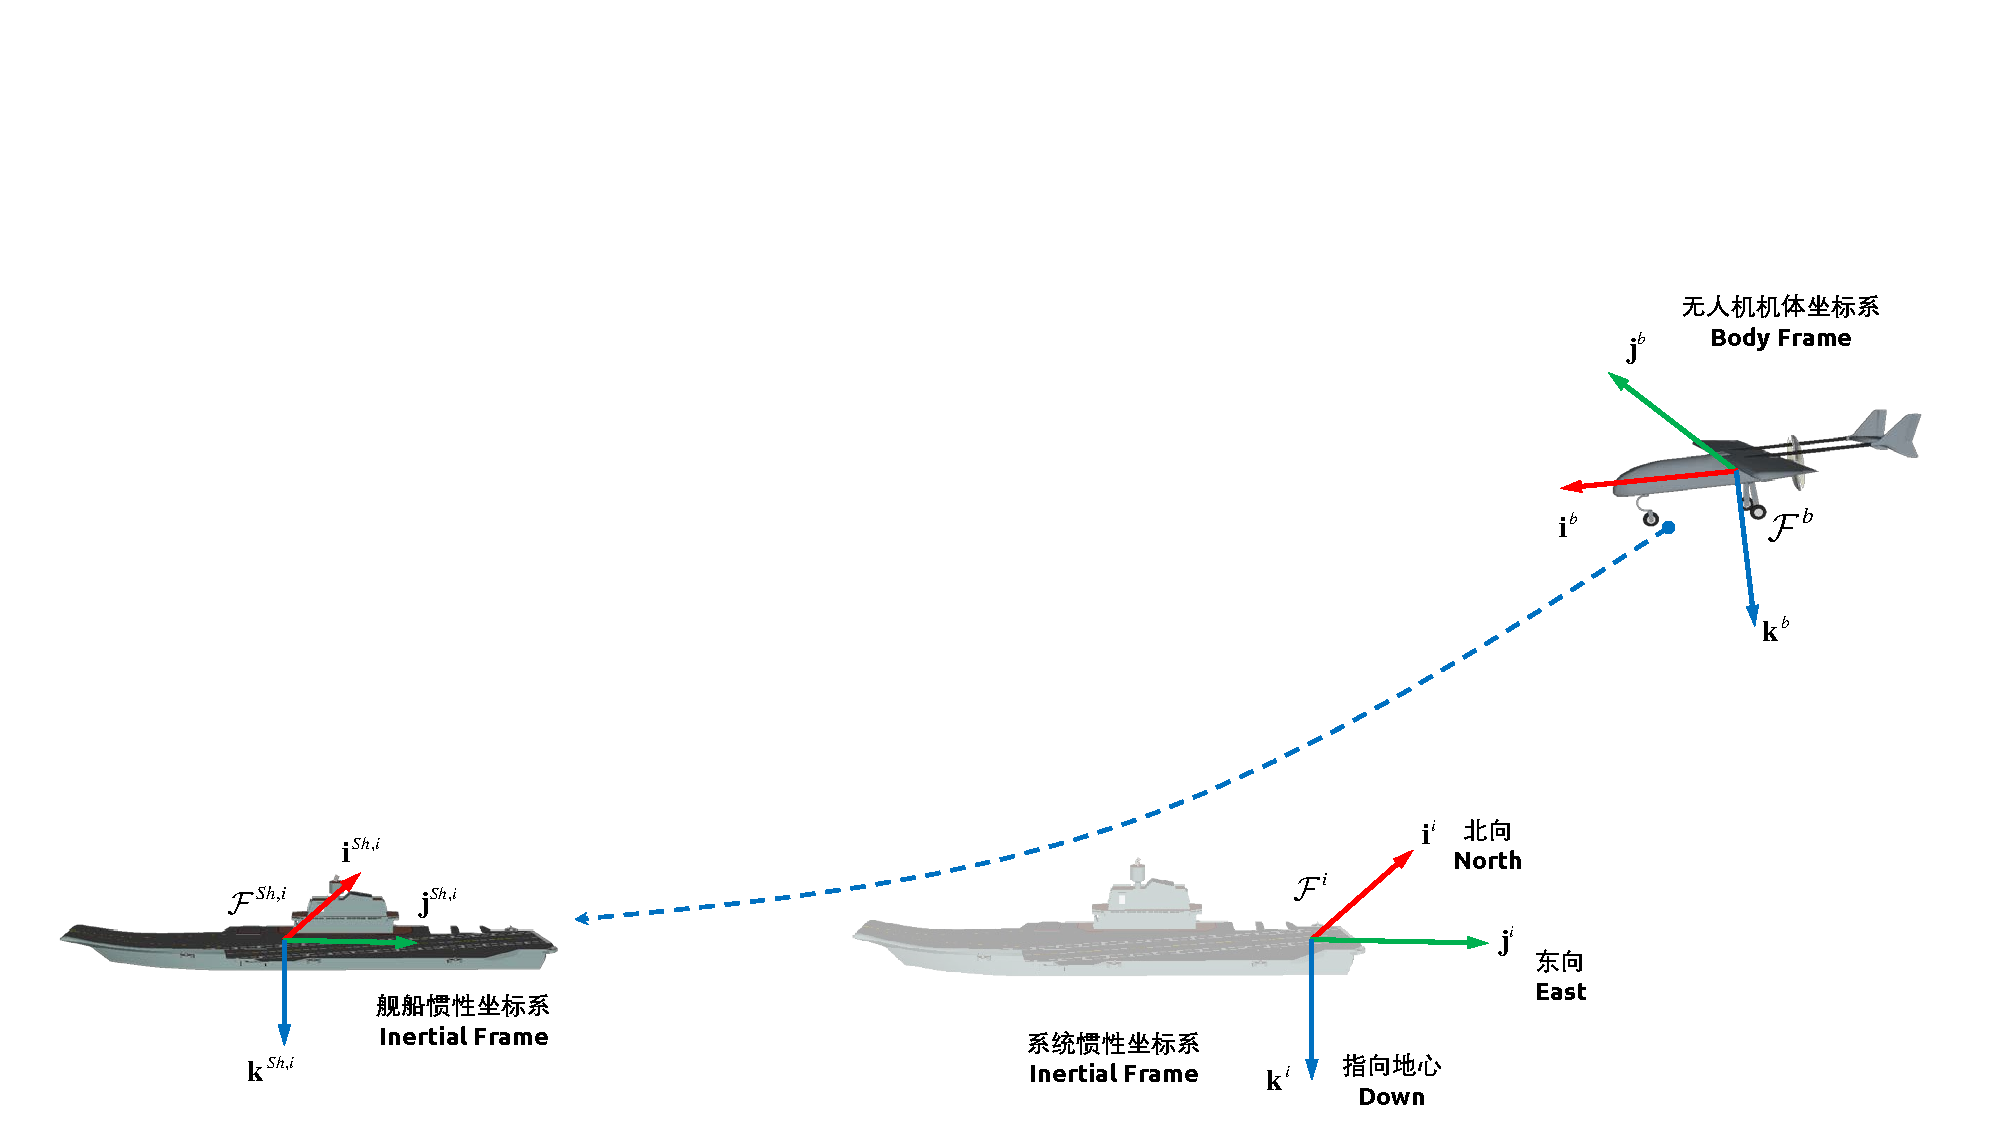
\includegraphics[width=\textwidth]{figs/chp02/chp02_01_sys_interial_frame.pdf}
	\caption{系统惯性坐标系}
	\label{fig:chp02_01_sys_interial_frame}
\end{figure}

\subsection{无人机惯性坐标系}
无人机惯性坐标系($\mathcal{F}^v$,Vehicle Inertial Frame),该坐标系的原点位于飞机的重心,三轴方向与系统坐标系平行。

\begin{figure}[tb]   
	\centering
	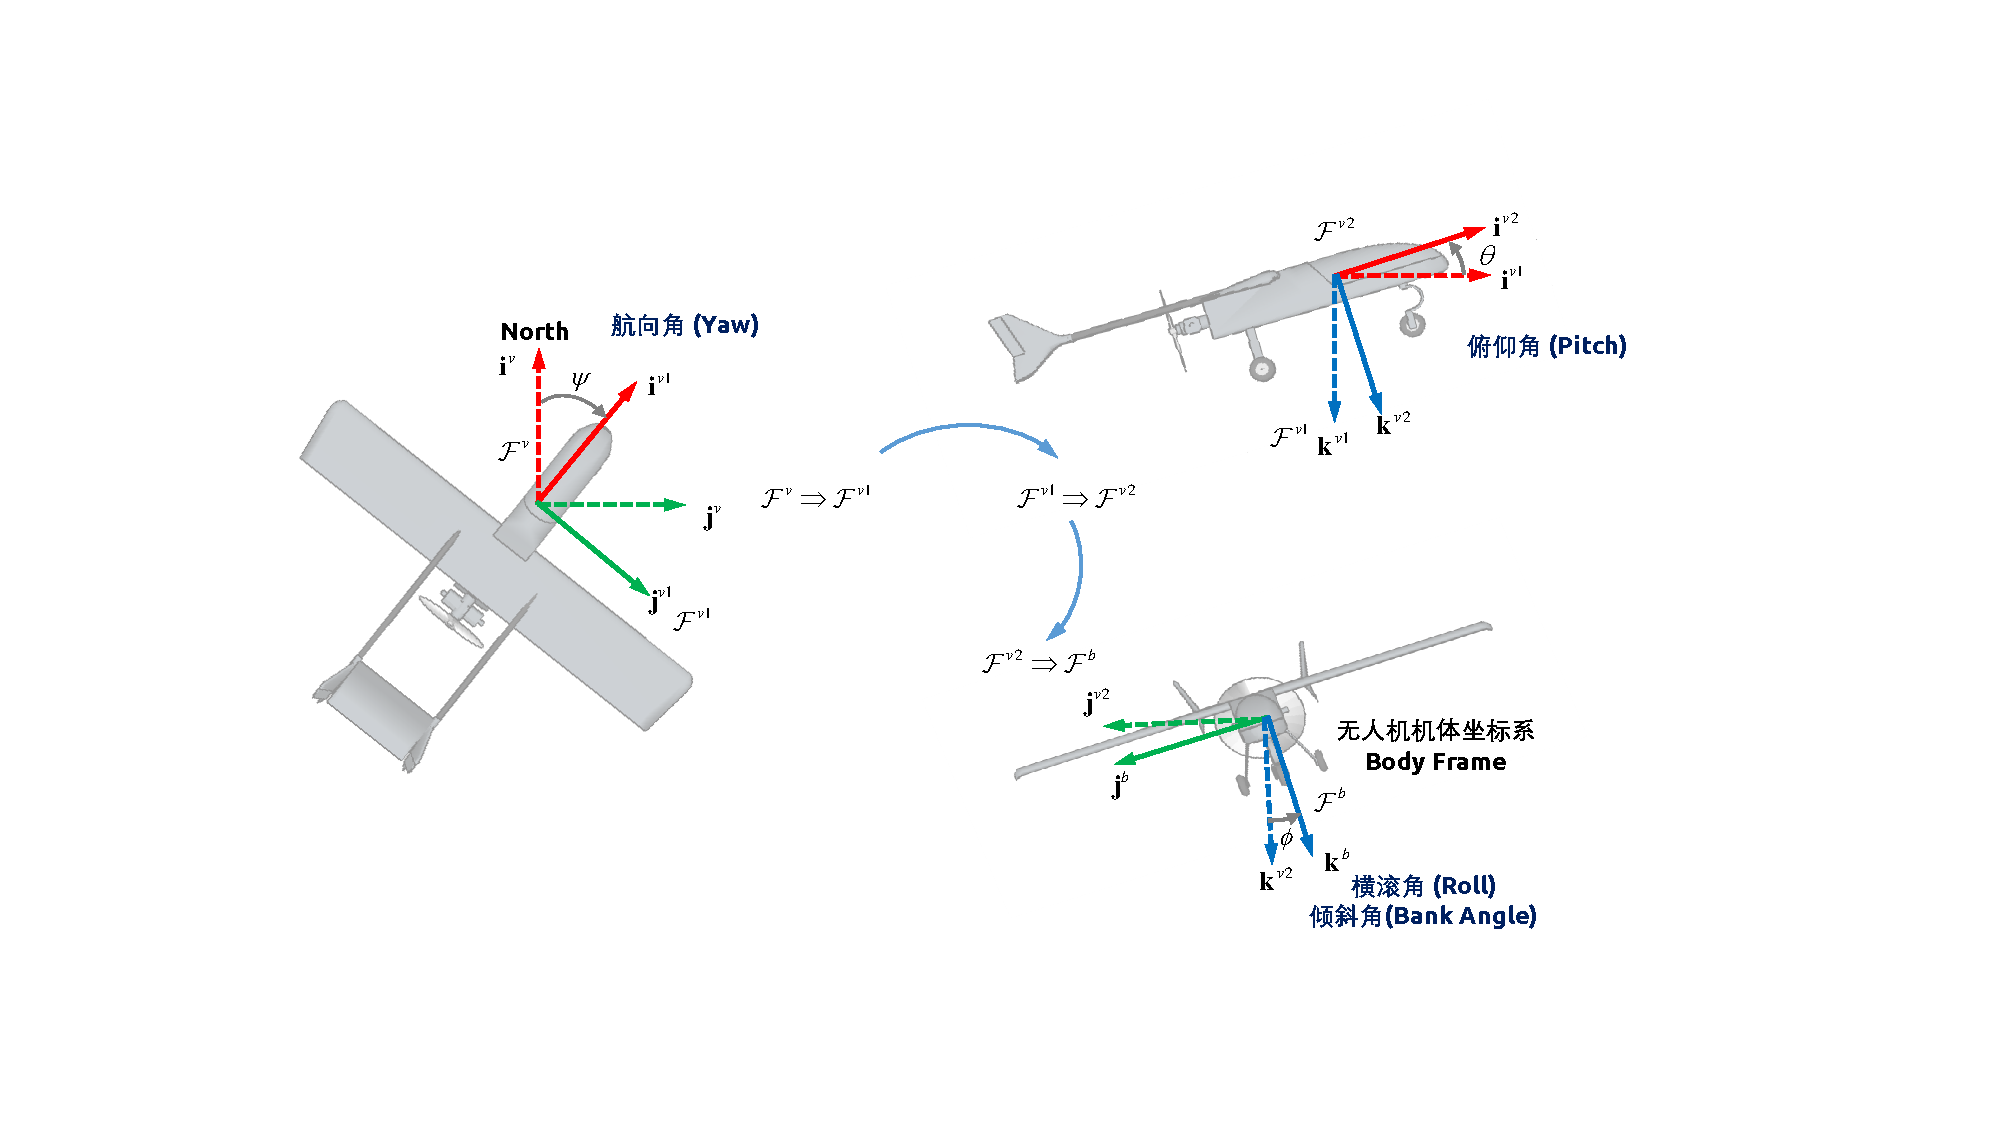
\includegraphics[width=\textwidth]{figs/chp02/chp02_02_uav_rpy.pdf}
	\caption{无人机机体坐标系与横滚角、俯仰角和偏航角定义}
	\label{fig:chp02_02_uav_rpy}
\end{figure}

无人机第一惯性辅助坐标系($\mathcal{F}^{v1}$ ),该坐标系绕无人机惯性坐标系$\mathbf{k}^v$轴按右手规则旋转得到,其中旋转角度定义为$\psi$,即偏航角(Yaw Angle)。

无人机第二惯性辅助坐标系($\mathcal{F}^{v2}$),该坐标系过绕人机第一惯性辅助坐标系$\mathbf{j}^{v1}$轴按右手规则旋转旋转得到,其旋转角度定义为$\theta$,即俯仰角(Pitch Angle)。

无人机机体坐标系($\mathcal{F}^b$,Body Frame ),该坐标系绕无人机第二惯性辅助坐标系$\mathbf{i}^{v2}$轴按右手规则旋转旋转得到,其旋转角度定义为$\phi$,即横滚角(Roll Angle),有时该角度也被称为倾斜角(Bank Angle)。上述四个坐标系之间的转换关系如图\ref{fig:chp02_02_uav_rpy}所示。

根据上述四个坐标系的几何关系,可以得到由机体惯性坐标系$\mathcal{F}^v$转换到机体坐标系$\mathcal{F}^b$的转换矩阵为
\begin{multline}
	\mathcal{R}_v^b(\phi, \theta, \psi) =\mathcal{R}_{v2}^b(\phi)\mathcal{R}_{v1}^{v2}(\theta)\mathcal{R}_v^{v1}(\psi) \\
	=\begin{bmatrix}
		\cos \theta \cos \psi                             & \cos\theta \sin\psi                               & -\sin\theta         \\
		-\cos\phi \sin\psi + \sin\phi \sin\theta \cos\psi & \cos\phi \cos\psi + \sin\phi \sin\theta\sin\psi   & \sin\phi \cos\theta \\
		\sin\phi \sin\psi + \cos\phi \sin\theta \cos\psi  & -\sin\phi \cos\psi + \cos\phi \sin\theta \sin\psi & \cos\phi \cos\theta
	\end{bmatrix}
\end{multline}





机体坐标系$\mathcal{F}^b$转换到稳定坐标系$\mathcal{F}^s$的转换矩阵为
\begin{equation} 
	\mathcal{R}_b^s(\alpha) = \begin{bmatrix}
		\cos \alpha                             & 0                               & \sin \alpha         \\
		0 & 1   &0 \\
		-\sin \alpha   & 0 & \cos \alpha
	\end{bmatrix}
\end{equation}

稳定坐标系$\mathcal{F}^s$转换为风坐标系$\mathcal{F}^w$的转换矩阵为
\begin{equation} 
	\mathcal{R}_s^w(\beta) = \begin{bmatrix} \sin \beta  & \cos \beta  &  0      \\  - \sin \beta & \cos \beta   &0 \\  0   & 0 &1  \end{bmatrix}
\end{equation}

风坐标系$\mathcal{F}^w$转换为机体坐标系$\mathcal{F}^b$转换矩阵为

\begin{equation} 
	\mathcal{R}_w^b (\alpha,\beta) = \begin{bmatrix} \cos \beta \cos \alpha & - \sin \beta \cos \alpha  & - \sin \alpha      \\	 \sin \beta & \cos \beta   & 0 \\	\cos \beta   & -\sin \beta \sin \alpha & \cos \alpha \end{bmatrix}
\end{equation}

\subsection{无人机风向坐标系}
无人机风向坐标系($\mathcal{F}^w$,Wind Frame),该坐标系的$\mathbf{i}^w$轴与风速方向相同,可以通过旋转稳定坐标系的$\mathbf{k}^s$轴$\beta$角度得到,该角度$\beta$被定义为侧滑角。无人机攻角和侧滑角的定义如图\ref{fig:chp02_03_uav_aoa_bank}所示。
\begin{figure}[tb]   
	\centering
	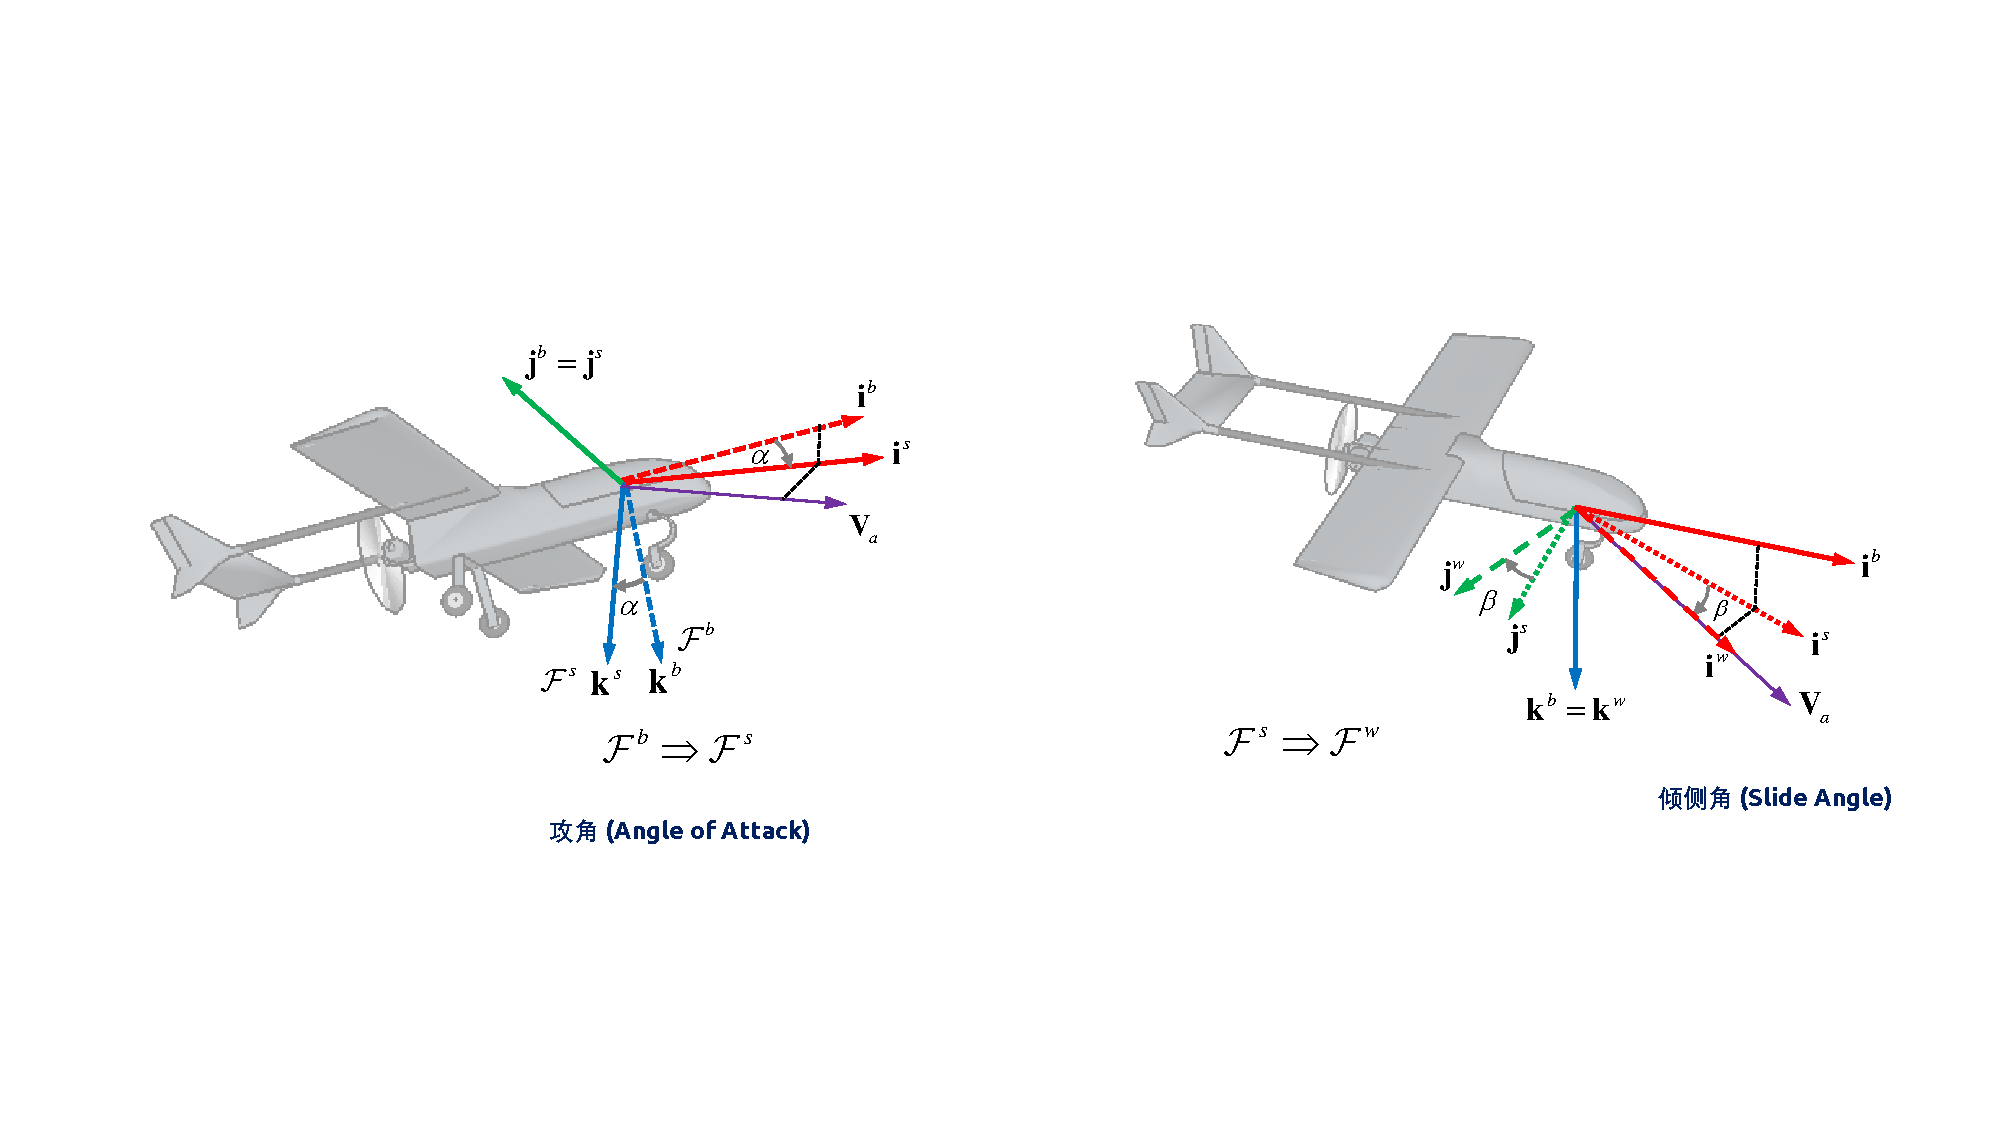
\includegraphics[width=\textwidth]{figs/chp02/chp02_03_uav_aoa_bank.pdf}
	\caption{无人机稳定坐标系与攻角、侧滑角定义}
	\label{fig:chp02_03_uav_aoa_bank}
\end{figure}

\subsection{无人机稳定坐标系}
无人机稳定坐标系($\mathcal{F}^s$,Stability Frame),该坐标系绕无人机机体坐标系$\mathbf{j}^b$按左手规则旋转得到,该坐标系表达如图\ref{fig:chp02_03_uav_aoa_bank}。其中,定义无人机相对于机体周边空气的速度向量为$\mathbf{V}_a$,其大小为$V_a$。为使机翼产生升力,机翼与风速的夹角必须为正,该角度定义为攻角。这里使用左手系的原因是为更方便的定义定义攻角$\alpha$的正负,即沿稳定坐标系$\mathbf{j^s}$按右手系转动到机体坐标系的角度为正。稳定坐标系的$\mathbf{i}^s$轴与空速向量$\mathbf{V}_a$在$\mathbf{i}^b$-$\mathbf{k}^b$的投影方向平行。

定义$\mathbf{V}_a$为空速(Airspeed),即无人机相对于周边流体的速度。
该向量在风坐标系$\mathcal{F}^w$的表达为
\begin{equation} 
	\mathbf{V}_a^w=\begin{bmatrix} V_a \\ 0 \\ 0 \end{bmatrix}
\end{equation}
该向量在机体坐标系$\mathcal{F}^b$的表达为
\begin{equation} 
	\mathbf{V}_a^b = \begin{bmatrix} u_r \\ v_r \\ w_r \end{bmatrix}
\end{equation}

$\mathbf{V}_g$定义为地速(Ground Speed),即无人机相对于系统惯性系的速度
无人机相对于惯性系的速度该向量在机体坐标系$\mathcal{F}^b$的表达为
\begin{equation}
	\mathbf{V}_g^b=\begin{bmatrix} u \\ v \\w \end{bmatrix}
\end{equation}

$\mathbf{V}_w$定义为风速(Wind Speed),即风相对于系统惯性系的速度。
风速在机体坐标系$\mathcal{F}^b$的表达为
\begin{equation}
	\mathbf{V}_w^b=\begin{bmatrix} u_w \\ v_w \\w_w \end{bmatrix} \\
	=\mathcal{R}_v^b(\phi, \theta, \psi) \begin{bmatrix} w_n \\ w_e \\ w_d \end{bmatrix}
\end{equation}
其中$(w_n, w_e, w_d)$是风速在无人机惯性坐标系的表达。
上述三个速度直接的关系为
\begin{equation}
	\mathbf{V}_a = \mathbf{V}_b - \mathbf{V}_w
\end{equation}

上述三个关系的表达如图\ref{fig:chp02_04_uav_wind_frame}所示,根据上述关系,可以得到风速在机体坐标系的另一个表达
\begin{equation}
	\mathbf{V}_a^b  = \begin{bmatrix} u_r \\ v_r \\ w_r \end{bmatrix} =   \begin{bmatrix} u - u_w \\ v - v_w \\ w- w_w \end{bmatrix}
\end{equation}
根据风坐标系$\mathcal{F}^w$与$\mathcal{F}^b$机体坐标系的转换关系,风速在机体坐标系还可以表达为
\begin{equation}
	\mathbf{V}_a^b  = \begin{bmatrix} u_r \\ v_r \\ w_r \end{bmatrix} \\
	=  \mathcal{R}_w^b \begin{bmatrix} V_a \\ 0 \\ 0 \end{bmatrix} \\
	=  \begin{bmatrix}	\cos \beta \cos \alpha & - \sin \beta \cos \alpha  & - \sin \alpha      \\	 \sin \beta & \cos \beta   & 0 \\ 	\cos \beta   & -\sin \beta \sin \alpha & \cos \alpha \end{bmatrix} \begin{bmatrix} V_a \\ 0 \\ 0 \end{bmatrix}
\end{equation}
由此可以得到上式更简便的表达
\begin{equation}
	\begin{bmatrix} u_r \\ v_r \\ w_r \end{bmatrix}  = {V}_a \begin{bmatrix} \cos \alpha \cos \beta \\ \sin \beta  \\ \sin \alpha \cos \beta \end{bmatrix}
\end{equation}
注意,此处的$V_a$是风速向量的标量。

在已知风速相对于机体坐标系的向量表达时,可以进一步得到风速、攻角和侧滑角的计算
\begin{align}
	V_a &= \sqrt{(u_r)^2+(v_r)^2+(w_r)^2} \\
	\alpha &=  \tan^{-1}\frac{w_r}{u_r}  \\
	\beta  &=  \sin^{-1} \big( \frac{u_r}{\sqrt{(u_r)^2+(v_r)^2+(w_r)^2}} \big)
\end{align}

\begin{figure}[htb]   
	\centering
	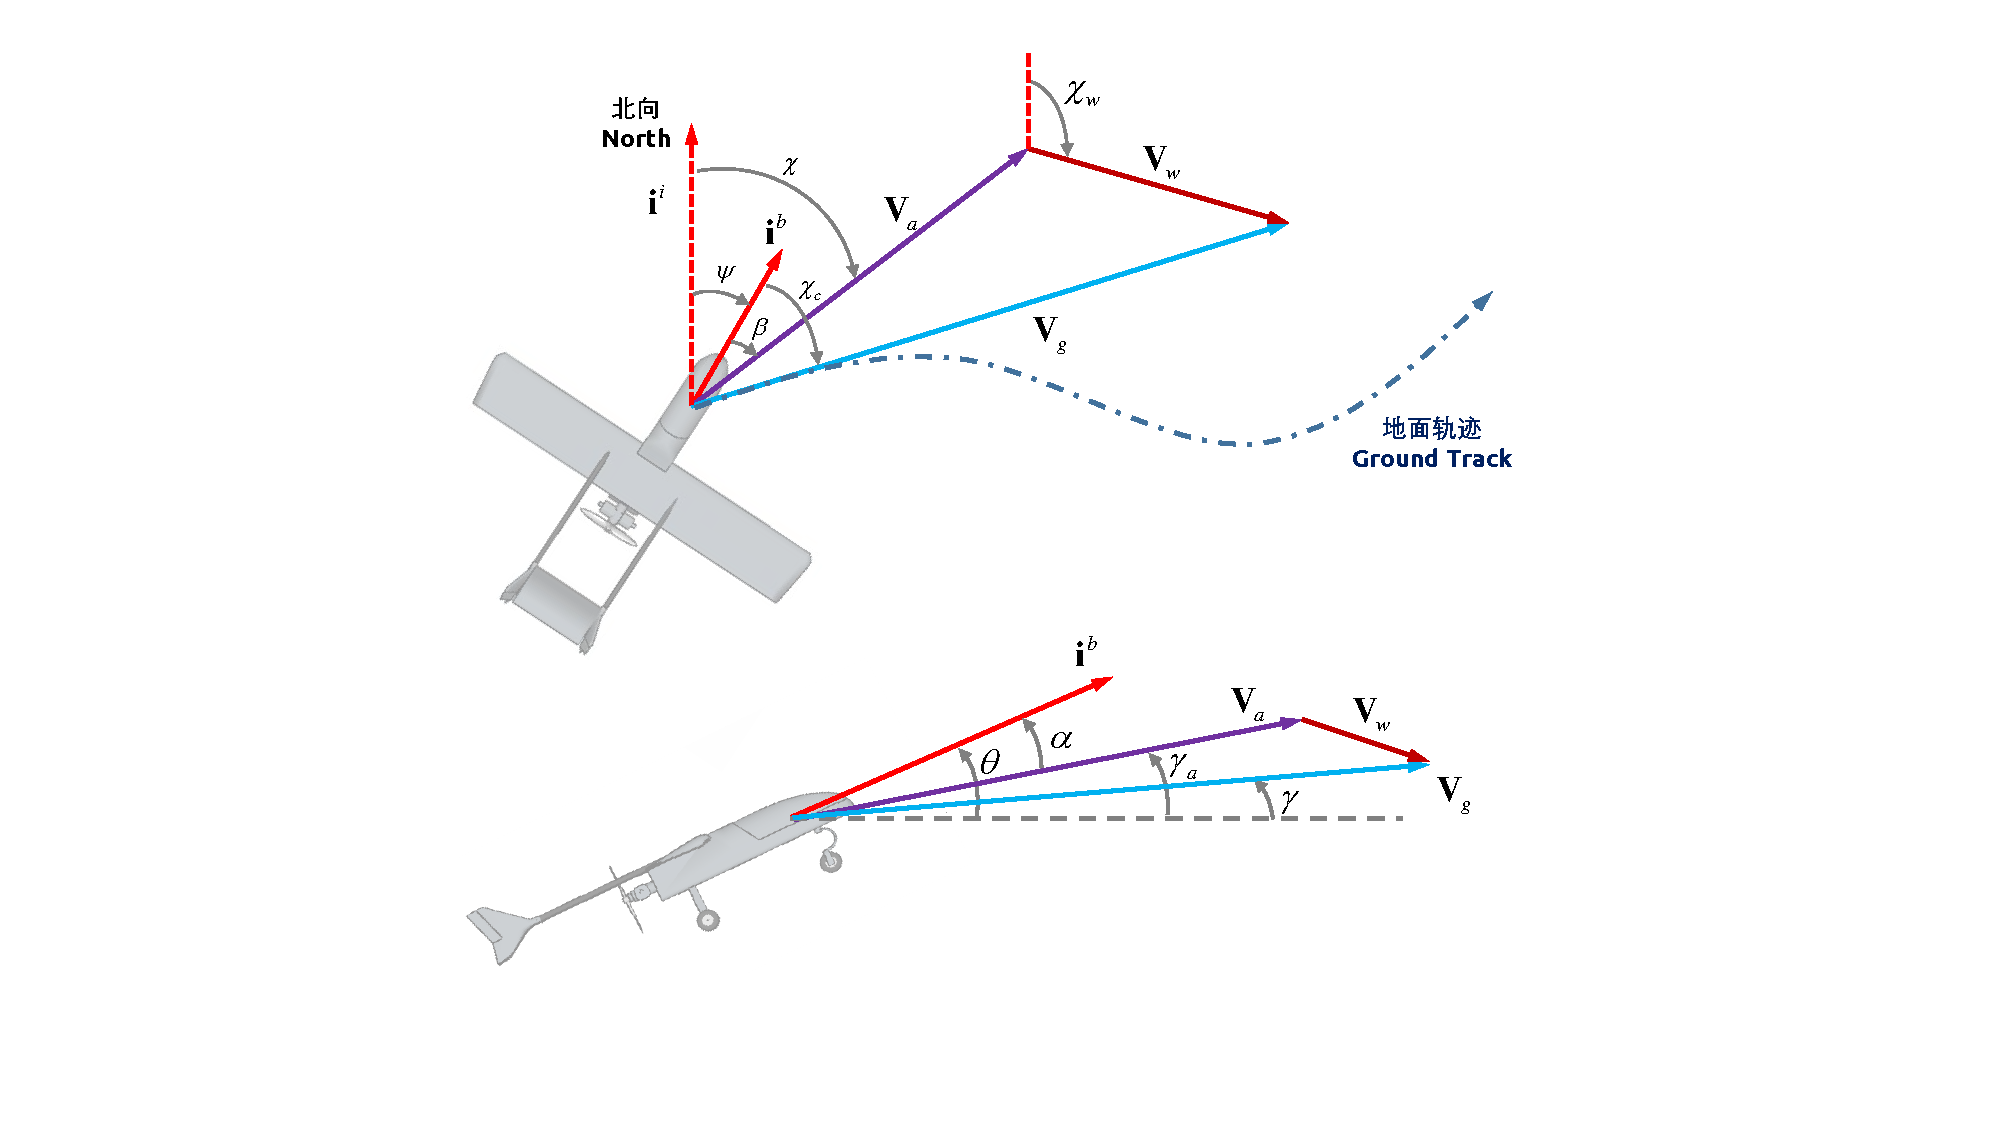
\includegraphics[width=0.8\textwidth]{figs/chp02/chp02_04_uav_wind_frame.pdf}
	\caption{无人机地速、风速和空速三角形}
	\label{fig:chp02_04_uav_wind_frame}
\end{figure}






\subsection{三维空间向量微分}
假设在机体坐标系$\mathcal{F}^b$存在一个运动的向量$\mathbf{p}$,如图\ref{fig:chp02_06_vector_rotation}所示,该向量的数学表达为 
\begin{equation}
	\mathbf{p }= p_x \mathbf{i}^b +  p_y \mathbf{j}^b +  p_z \mathbf{k}^b
\end{equation}
\begin{figure}[htb]   
	\centering
	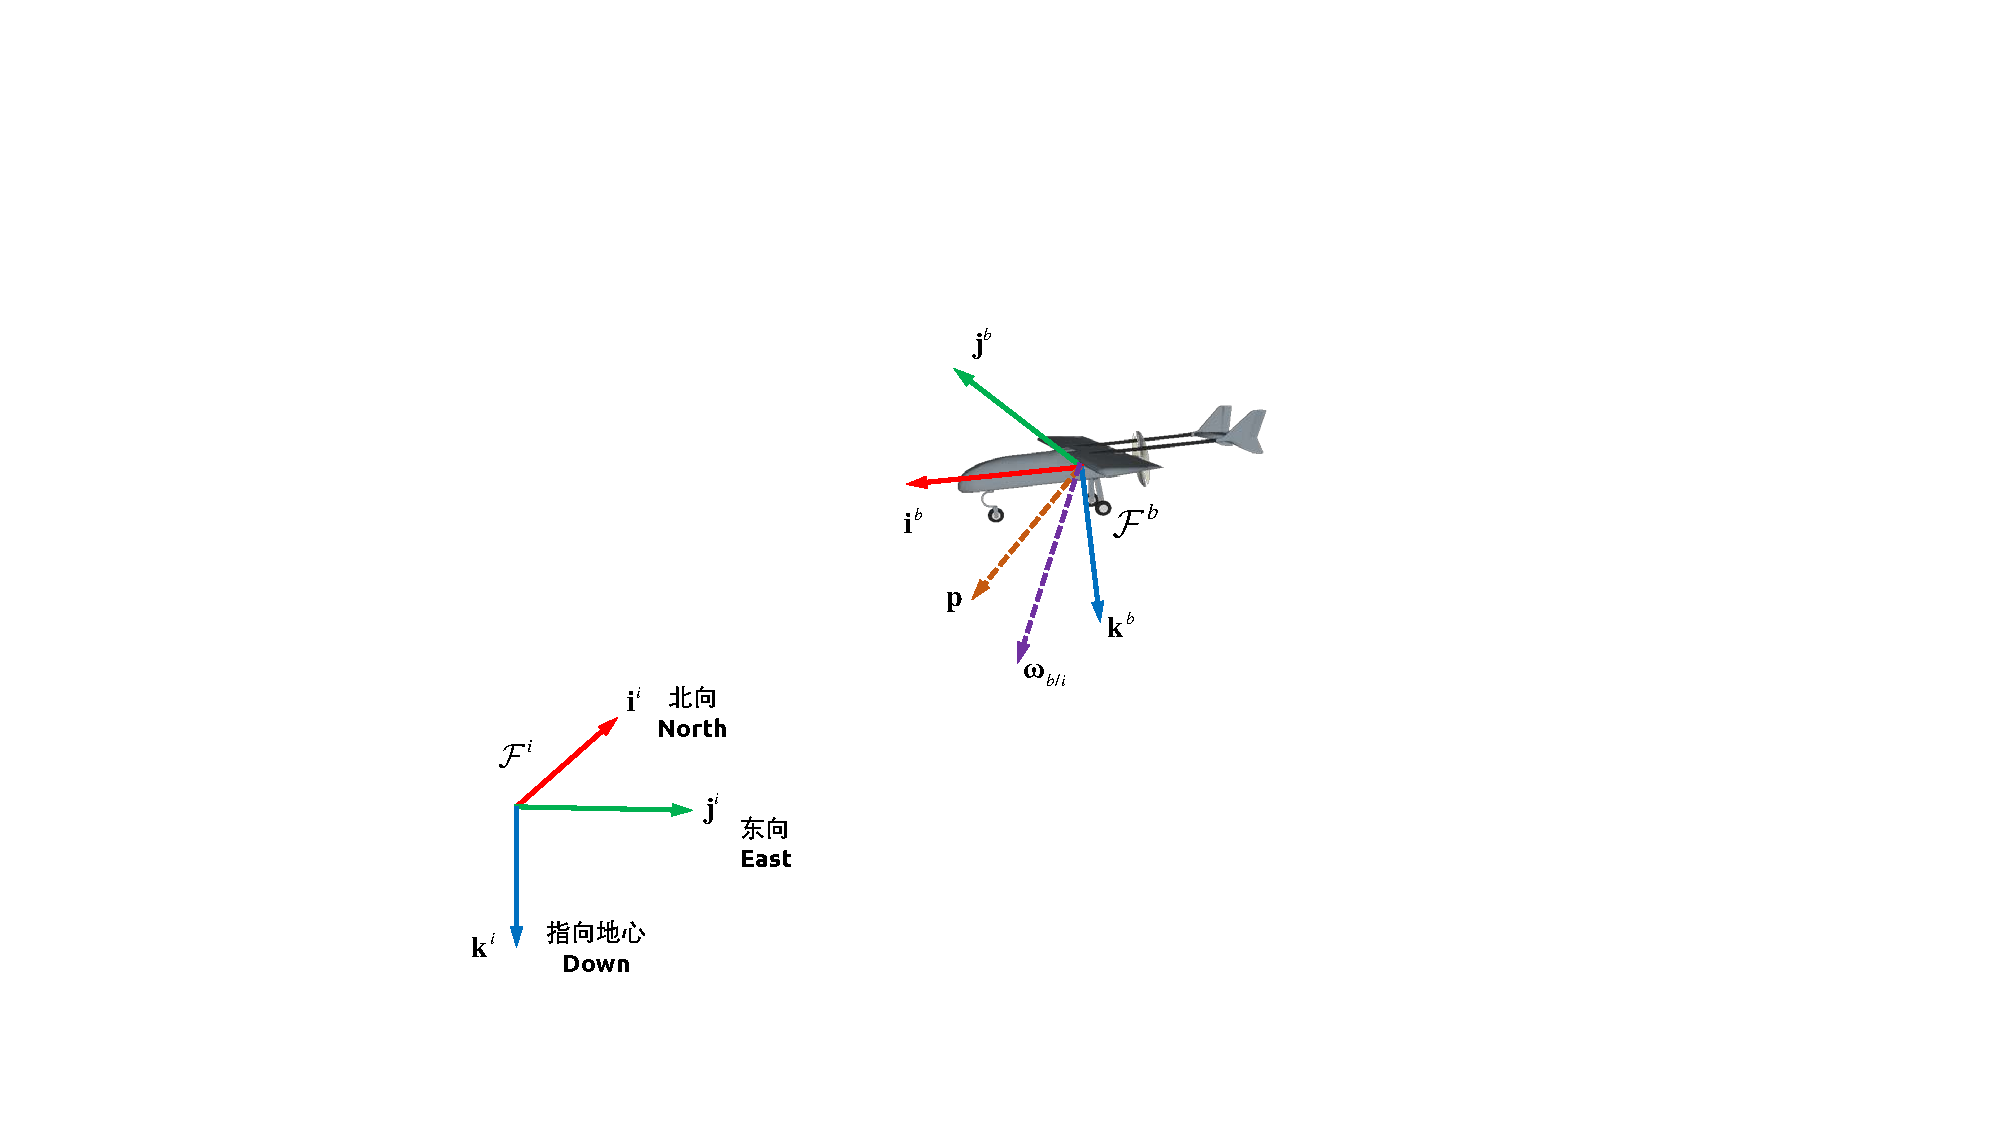
\includegraphics[width=0.8\textwidth]{figs/chp02/chp02_06_vector_rotation.pdf}
	\caption{三维空间向量微分}
	\label{fig:chp02_06_vector_rotation}
\end{figure}

此时机体坐标系$\mathcal{F}^b$与惯性坐标系$\mathcal{F}^i$只存绕转动向量$\mathbf{\omega}_{b/i}$的转动,不存在平动。由此得到该运动向量$\mathbf{p}$相对于系统坐标系$\mathcal{F}^i$的微分为
\begin{equation} \label{chp02_vector_derivative}
	\frac{d}{dt_i} \mathbf{p} = \frac{d}{dt_b} \mathbf{p} + \mathbf{\omega}_{b/i} \times \mathbf{p}
\end{equation}
其中等式右侧的第一项具体表达为
\begin{equation}
	\frac{d}{dt_i} \mathbf{p} = \dot{p}_x \mathbf{i}^b +  \dot{p}_y \mathbf{j}^b +  \dot{p}_z \mathbf{k}^b
\end{equation}
该部分可以通过设计无人机状态的观测器的获得。

\subsection{无人机空间位置定义}
因为飞机着舰过程的运动范围相对较小,由此对问题的坐标的整体构架主要选用Flat-Earth模型来替代WGS-84模型。首先,对于无人机在系统惯性系$\mathcal{F}^i$的位置定义为$(p_n\ p_e\ p_d)^T$,其中$n$, $e$  和$d$ 描述系统坐标系正北、正东和指向地心的方向。定义$h = -p_d$,用于描述无人机的飞行高度。无人机在系统惯性系的速度在机体坐标系$\mathcal{F}^b$的投影为$(u, v, w)$,无人机在机体坐标系$\mathcal{F}^b$的旋转角速度为$(p, q, r)$。则可以得到无人机速度在两个坐标系的相互转换关系
\begin{equation}
	\frac{d}{dt} \begin{bmatrix} p_n \\ p_e \\ p_d \end{bmatrix}   =  (\mathcal{R}_v^b)^T \begin{bmatrix} u \\  v \\ w \end{bmatrix}  
\end{equation}
\begin{equation}
	\resizebox{.9 \textwidth}{!} 
	{ $
		\begin{bmatrix} \dot{p}_n \\ \dot{p}_e \\ \dot{p}_d \end{bmatrix} = \begin{bmatrix}  cos \theta \cos \psi   &     -\cos\phi \sin\psi + \sin\phi \sin\theta \cos\psi                        &  \sin\phi \sin\psi + \cos\phi \sin\theta \cos\psi       \\
		\cos\theta \sin\psi    & \cos\phi \cos\psi + \sin\phi \sin\theta\sin\psi   & -\sin\phi \cos\psi + \cos\phi \sin\theta \sin\psi \\
		-\sin\theta  & \sin\phi \cos\theta & \cos\phi \cos\theta
		\end{bmatrix} \begin{bmatrix} u \\  v \\ w \end{bmatrix}
		$}
\end{equation}
进一步化解可以得到
\begin{align}
	\begin{bmatrix} p \\ q \\ r \end{bmatrix}  &=   \begin{bmatrix}
		1 &  0   & -\sin \theta      \\
		0 &  \cos \phi  & \sin \phi \cos \theta \\	
		0 & -\sin \phi   & \cos \phi \cos \theta
	\end{bmatrix} \begin{bmatrix} \dot{\phi} \\ \dot{\theta} \\ \dot{\psi} \end{bmatrix} \\
	\begin{bmatrix} \dot{\phi} \\ \dot{\theta} \\ \dot{\psi} \end{bmatrix}  &=  \begin{bmatrix}
		1 &  \sin \phi \tan \theta  & - \cos \phi \tan \theta      \\
		0 & \cos \phi   & -\sin \phi \\
		0  & \sin \phi \sec \theta & \cos \phi \sec \theta
	\end{bmatrix} \begin{bmatrix} p \\ q \\ r \end{bmatrix}
\end{align}

\subsection{无人机的外部力和力矩分析}
无人机的质量定义为$\mathsf{m}$,所受全部外力定义为$\mathbf{f}$,主要由重力$\mathbf{f}_g$、空气动力$\mathbf{f}_a$和电机拉力$\mathbf{f}_p$三部分组成
\begin{equation}
	\mathbf{f} = \mathbf{f}_g + \mathbf{f}_a + \mathbf{f}_p
\end{equation}

重力在无人机惯性坐标系$\mathcal{F}^v$的表达为
\begin{equation}
	\mathbf{f}_g^v = \begin{bmatrix}0  \\ 0  \\ \mathsf{m}g  \end{bmatrix}
\end{equation}

重力在无人机机体坐标系$\mathcal{F}^b$的表达为
\begin{equation}
	\mathbf{f}_g^b =\mathcal{R}^b_v \begin{bmatrix}0  \\ 0  \\ \mathsf{m}g  \end{bmatrix} \\
	= \begin{bmatrix} -\mathsf{m} g \sin \theta  \\ \mathsf{m}g \cos \theta \sin \phi  \\ \mathsf{m}g \cos\theta \cos \phi  \end{bmatrix}
\end{equation}

根据空气动力定义,在水平方向,无人机受到的升力$F_{lift}$、阻力$F_{drag}$和力矩$m$,其基本定义为
\begin{align}
	F_{filt} = \frac{1}{2} V_a^2SC_L(\alpha, q, \delta_e) \\
	F_{drag} = \frac{1}{2} V_a^2SC_D(\alpha, q, \delta_e) \\
	m = \frac{1}{2} V_a^2ScC_m(\alpha, q, \delta_e)
\end{align}
其中$S$是机翼面积,$c$是机翼平均舷长,$C_L$、$C_D$和$C_m$是非线性空气动力参数。此外,无人机的控制面为三个,副翼偏移$\delta_a$,方向舵偏移$\delta_r$和升降舵偏移$\delta_e$。

根据本文目标无人机的空气特性,由此将上述气动力参数进一步展开为
\begin{align}
	C_L(\alpha, q, \delta_e) &= C_X(\alpha) + {C_X}_q(\alpha) \frac{c}{2V_a}  q+ C_{X_{{\delta}_e}}(\alpha) \delta_e \\
	C_D(\alpha, q, \delta_e) &= C_{Y_{0}} + C_{Y_{\beta}} \beta + C_{Y_r}(\alpha) \frac{b}{2V_a} r+ C_{Y_{\delta_\alpha}} \delta_\alpha +  C_{Y_{\delta_r}} \delta_r  \\ 
	C_m(\alpha, q, \delta_e) &= C_Z(\alpha) + C_{Z_q}(\alpha) \frac{c}{2V_a}  q+ C_{Z_{\delta_e}} \delta_e
\end{align}
其中
\begin{align}
	C_X(\alpha) &= -C_D(\alpha) \cos \alpha +  C_L(\alpha) \sin \alpha \\
	C_{X_q}(\alpha) &= -C_{D_q} \cos \alpha +  C_{L_q} \sin \alpha \\
	C_{X_{\delta_e}}(\alpha) &= -C_{D_{\delta_e}} \cos \alpha +  C_{L_{\delta_e}} \sin \alpha \\
	C_Z(\alpha) &= -C_D(\alpha) \cos \alpha -  C_L(\alpha) \sin \alpha \\
	C_X(\alpha) &= -C_{D_q} \sin \alpha -  C_{L_q} \cos \alpha \\
	C_X(\alpha) &= -C_{D_{\delta_e}}  \sin \alpha -  C_{L_{\delta_e}} \cos \alpha \\
\end{align}
因为升力和阻力作用在无人机稳定坐标系$\mathcal{F}^s$上,因此将上述力转换到无人机的机体坐标系后,进一步得到
\begin{align}
	\begin{bmatrix} f_x    \\ f_z  \end{bmatrix} = \begin{bmatrix}
		\cos \alpha    & - \sin \alpha  \\
		\sin \alpha       & \cos \alpha  \\
	\end{bmatrix} \begin{bmatrix} -F_{drag}    \\ -F_{lift}  \end{bmatrix}
\end{align}
在竖直方向,无人机受到竖直方向的力和力矩为
\begin{align}
	f_y = \frac{1}{2} \rho V_a^2 S C_y (\beta, p, r, \delta_a, \delta_r) \\
	l  = \frac{1}{2} \rho V_a^2 S b  C_l (\beta, p, r, \delta_a, \delta_r) \\
	n = \frac{1}{2} \rho V_a^2 S b C_n (\beta, p, r, \delta_a, \delta_r)
\end{align}
其中,$C_y$、$C_l$和$C_n$是非线性空气动力参数。

螺旋桨的推力建模为
\begin{equation}
	\mathbf{f}_p = \frac{1}{2} \rho S_{prop} C_{prop}  \begin{bmatrix} (\mathsf{k}_{motor} \delta_t)^2 - V_a^2  \\ 0  \\ 0  \end{bmatrix}
\end{equation}
其中$\mathsf{k}_{motor}$是电机效率常数,$\delta_t$是电机的控制量,$S_{prop}$是螺旋桨的面积,$C_{prop}$是螺旋桨参数。

螺旋桨的力矩建模为
\begin{equation}
	\mathbf{T}_p = -\mathsf{k}_{T_p} (\mathsf{k}_{\Omega} \delta_{t})^2
\end{equation}

其中$\Omega = \mathsf{k}_{\Omega} \delta_{t}$是螺旋桨的转速,$\mathsf{k}_{T_p}$是电机常数。

\subsection{无人机的平动分析}
对于无人机的平动,无人机的质量为$\mathsf{m}$和其受到的全部外力$\mathbf{f}$,根据顿第二定律可以得到
\begin{equation}
	\mathsf{m} \frac{d \mathbf{V}_g}{d t_i} = \mathbf{f}
\end{equation}
代入\ref{chp02_vector_derivative}公式,可以得到
\begin{equation}
	\mathsf{m}(\frac{d \mathbf{V}_g }{dt_b}+ \mathbf{\omega}_{b/i} \times \mathbf{V}_g)=\mathbf{f}
\end{equation}
同理,在机体坐标系$\mathcal{F}^b$可以得到
\begin{equation}
	\mathsf{m}(\frac{d \mathbf{V}^b_g }{dt_b}+ \mathbf{\omega}_{b/i}^b \times \mathbf{V}^b_g)=\mathbf{f}^b
\end{equation}
其中$\mathbf{V}_g^b=(u, v, w)^T$描述无人机惯性系的速度向量在机体坐标系的表达,$\frac{d \mathbf{V}_g }{dt_b}=(\dot{u}, \dot{v}, \dot{w})^T$描述无人机速度在机体坐标系的变化率,$\mathbf{\omega}_{b/i}^b=(p, q, r)^T$描述无人机机体坐标系的转动角速度,$\mathbf{f}^b = (f_x, f_y, f_z)^T$描述外部合力向量在机体坐标系的表达。进一步可以得到
\begin{equation}
	\begin{bmatrix} \dot{u} \\ \dot{v} \\ \dot{w}  \end{bmatrix} = \begin{bmatrix} rv-qw \\ pw-ru \\ qu-pv  \end{bmatrix} + \frac{1}{\mathsf{m}} \begin{bmatrix} f_x \\ f_y \\ f_z  \end{bmatrix}
\end{equation}



\subsection{无人机的转动分析}
对于无人机对转动,定义角动量$\mathbf{h}$和全部外力矩$\mathbf{m}$,由此可以得到
\begin{equation}
	\frac{ d \mathbf{h}}{d t_i}=\mathbf{m}
\end{equation}
同理,对上式求在惯性系的微分
\begin{equation}
	\frac{ d \mathbf{h}}{d t_i} = \frac{d\mathbf{h}}{dt_b} + \mathbf{\omega}_{b/i} \times \mathbf{h} = \mathbf{m}
\end{equation}
同理,在机体坐标系的表达为
\begin{equation}
	\frac{ d \mathbf{h}^b}{d t_i} = \frac{d\mathbf{h}^b}{dt_b} + \mathbf{\omega}^b_{b/i} \times \mathbf{h}^b = \mathbf{m}^b
\end{equation}
对于刚体来说,角动量的表达通过惯量矩阵$\mathbf{J}$来定义
\begin{equation}
	\mathbf{h}^b=\mathbf{J}  \mathbf{\omega}^b_{b/i}
\end{equation}
其中
\begin{align}
	\mathbf{J} =\begin{bmatrix}	\int(y^2 + z^2)~d\mathsf{m} & -\int xy \ d\mathsf{m}        & -\int xz~d\mathsf{m} \\	-\int xy~d\mathsf{m}        & \int(x^2 + z^2)~d\mathsf{m} & -\int yz~d\mathsf{m} \\	-\int xz~d\mathsf{m}        & -\int yz~d\mathsf{m}  & \int(x^2 + y^2)~d\mathsf{m} \end{bmatrix}
\end{align}
根据无人机机体的对称性,该矩阵可以化简为
\begin{align}
	\mathbf{J} = \begin{bmatrix}	J_x     & 0   & -J_{xz} \\	0       & J_y & 0       \\	-J_{xz} & 0   & J_z  \end{bmatrix}
\end{align}
改矩阵的逆为
\begin{align}
	\mathbf{J}^{-1}=\frac{\mathrm{adj}(\mathbf{J}) }{\mathrm{det}(\mathbf{J}) } = \begin{bmatrix}	J_z / \Gamma     & 0   & J_{xz}/ \Gamma \\	0       & 1/ \Gamma & 0       \\	J_{xz}/ \Gamma & 0   & J_z/ \Gamma \end{bmatrix}
\end{align}
其中$ \Gamma = J_xJ_z - J_{xz}^2$ 。

同时,定义上式中的分量
\begin{align}
	\dot{\mathbf{\omega}}^b_{b/i}=\frac{ d \mathbf{\omega}^b_{b/i}}{dt_b} = \begin{bmatrix} \dot{p} \\ \dot{q} \\ \dot{r}  \end{bmatrix}
\end{align}
该分量描述在机体坐标系角速度的变化率。

根据上述公式可以得到对角速度变化率的求解
\begin{equation}
	\dot{\mathbf{\omega}}^b_{b/i} = \mathbf{J}^{-1}[{- \mathbf{\omega}}^b_{b/i} \times (\mathbf{J{\mathbf{\omega}}^b_{b/i}})+\mathbf{m}^b]
\end{equation}
定义无人机力矩在机体坐标系的表达$\mathbf{m}^b = (l, m, n)$

则可以得到对角速度变化率的进一步表达
\begin{equation}
	\begin{bmatrix} \dot{p} \\ \dot{q} \\ \dot{r}  \end{bmatrix} =  \begin{bmatrix} \Gamma_1pq - \Gamma_2qr + \Gamma_3 l + \Gamma_4 n \\ \Gamma_5pr - \Gamma_6(p^2-r^2) + \frac{1}{Jy}m \\ \Gamma_7pq - \Gamma_1qr + \Gamma_4l + \Gamma_8 n  \end{bmatrix}
\end{equation}
其中各个分量的表达为
\begin{align}
	\Gamma_1 &= \frac{J_{xz}(J_x-J_y+J_z)}{\Gamma}  \\
	\Gamma_2 &= \frac{J_z(J_z-J_y) + J_{xz}^2}{\Gamma}  \\
	\Gamma_3 &= \frac{J_z}{\Gamma}  \\
	\Gamma_4 &= \frac{J_{xz}}{\Gamma}  \\
	\Gamma_5 &= \frac{J_z - J_x}{J_y}  \\
	\Gamma_6 &= \frac{J_{xz}}{J_y}  \\
	\Gamma_7 &= \frac{(J_x-J_z)J_x+J_{xz}^2}{\Gamma}  \\
	\Gamma_8 &= \frac{J_x}{\Gamma}  \\
\end{align}

\subsection{无人机运动轨迹数学描述}

\begin{figure}[htb]   
	\centering
	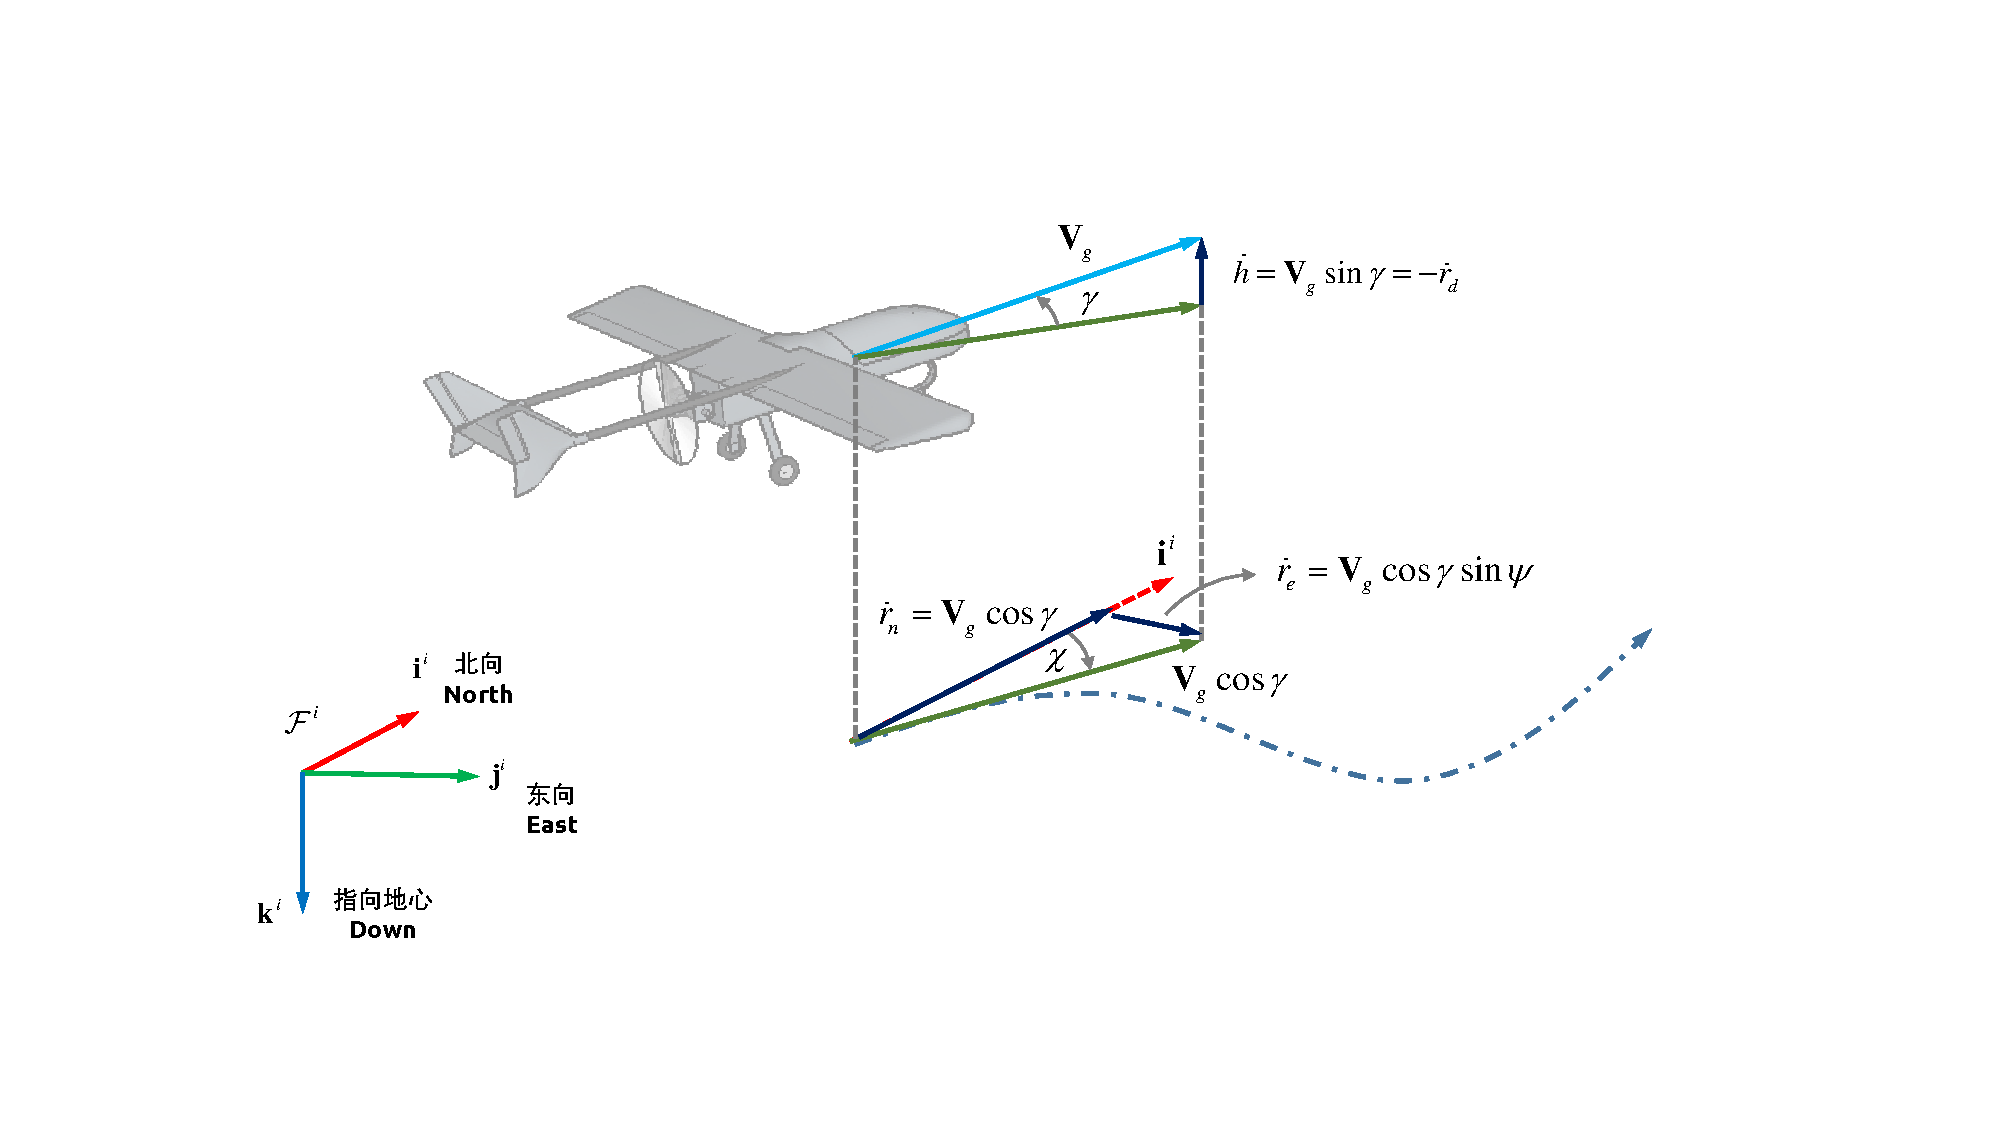
\includegraphics[width=0.8\textwidth]{figs/chp02/chp02_05_uav_course_frame.pdf}
	\caption{无人机运动轨迹描述}
	\label{fig:chp02_05_uav_course_frame}
\end{figure}

定义无人机在惯性系的坐标为$(p_n\ p_e\ p_d)^T$,无人机速度$\mathbf{V}_g$在惯性系的分量为$(\dot{p}_n\ \dot{p}_e\ \dot{p}_d)^T$,该速度的大小用$V_g = ||\mathbf{V}_g||$来表达,如图\ref{fig:chp02_05_uav_course_frame}所示。根据空间几何关系可以得到
\begin{equation}
	\begin{bmatrix} \dot{p}_n \\\dot{p}_e \\ \dot{p}_d \end{bmatrix}  = {V}_g \begin{bmatrix} \cos \psi \cos \gamma \\ \sin \psi \cos \gamma  \\- \sin \gamma \end{bmatrix}
\end{equation}
其中航迹角$\gamma$定义为地速$\mathbf{V}_g$与惯性系北向$\mathbf{i}^i$与动向$\mathbf{j}^i$所构成的地平面的夹角,航迹偏航角$\chi$定义为地速$\mathbf{V}_g$在地面投影与正北方向的夹角。

由于无人机受到的升力为$F_{lift}$,在无人机进行协调转弯(Coordinated Turn)时,根据力学关系可以得到横向和纵向公式
\begin{align}
	&F_{lift} \sin \phi \cos (\chi - \psi) = \mathsf{m} \frac{v^2}{R}  \\
	&F_{lift } \cos \phi = \mathsf{m} g \cos \gamma
\end{align}
将上述两式相除,并对$\chi$微分,可以得到
\begin{equation}
	\dot{\chi} = \frac{g}{V_g} \tan \phi \cos (\chi - \psi)
\end{equation}
在没有风速影响下($V_g = V_a\ , \psi = \chi$),可以将上式进一步化简为
\begin{equation}
	\dot{\psi} =\frac{g}{V_a} \tan \phi
\end{equation}
因为无人机的控制一般分为内环和外环,内环的控制速率较快,即飞行控制器可以很快使得无人机的姿态角收敛到指令期望位置,即$\gamma = \gamma^c\ , \phi = \phi^c$。因此,无人机的运动情况可以通过如下公式进一步描述
\begin{equation}
	\begin{bmatrix} \dot{p}_n \\\dot{p}_e \\ \dot{p}_d \end{bmatrix}  = {V}_a \begin{bmatrix} \cos \psi \cos \gamma^c \\ \sin \psi \cos \gamma^c  \\- \sin \gamma^c \end{bmatrix} \\
	\dot{\psi} =\frac{g}{V_a} \tan \phi^c
\end{equation}
由于无人机执行机构的物理约束,无人机的控制指令收到进一步约束
\begin{align}
	|\phi^c| \le \bar{\phi} \\
	|\gamma^c| \le \bar{\gamma}
\end{align}
其中$\bar{\phi}$和$\bar{\gamma}$为无人机系统的最大横滚角和下滑角约束。



舰船坐标系主要由舰船惯性坐标系、舰船龙骨坐标系和着舰点坐标系三部分组成。
\section{舰船系统坐标系定义}
\subsection{舰船惯性坐标系}
舰船惯性坐标系($\mathcal{F}^{Sh,i}$,Ship Inertial Frame),该坐标系的原点定义在舰船的中心位置,一般位于龙骨所在轴线,位于甲板下方。该坐标系的三个轴的方向分别与系统坐标系$\mathcal{F}^i$平行。该坐标系的表达如图\ref{fig:chp02_08_ship_interial_frame}所示。

\begin{figure}[htb]   
	\centering
	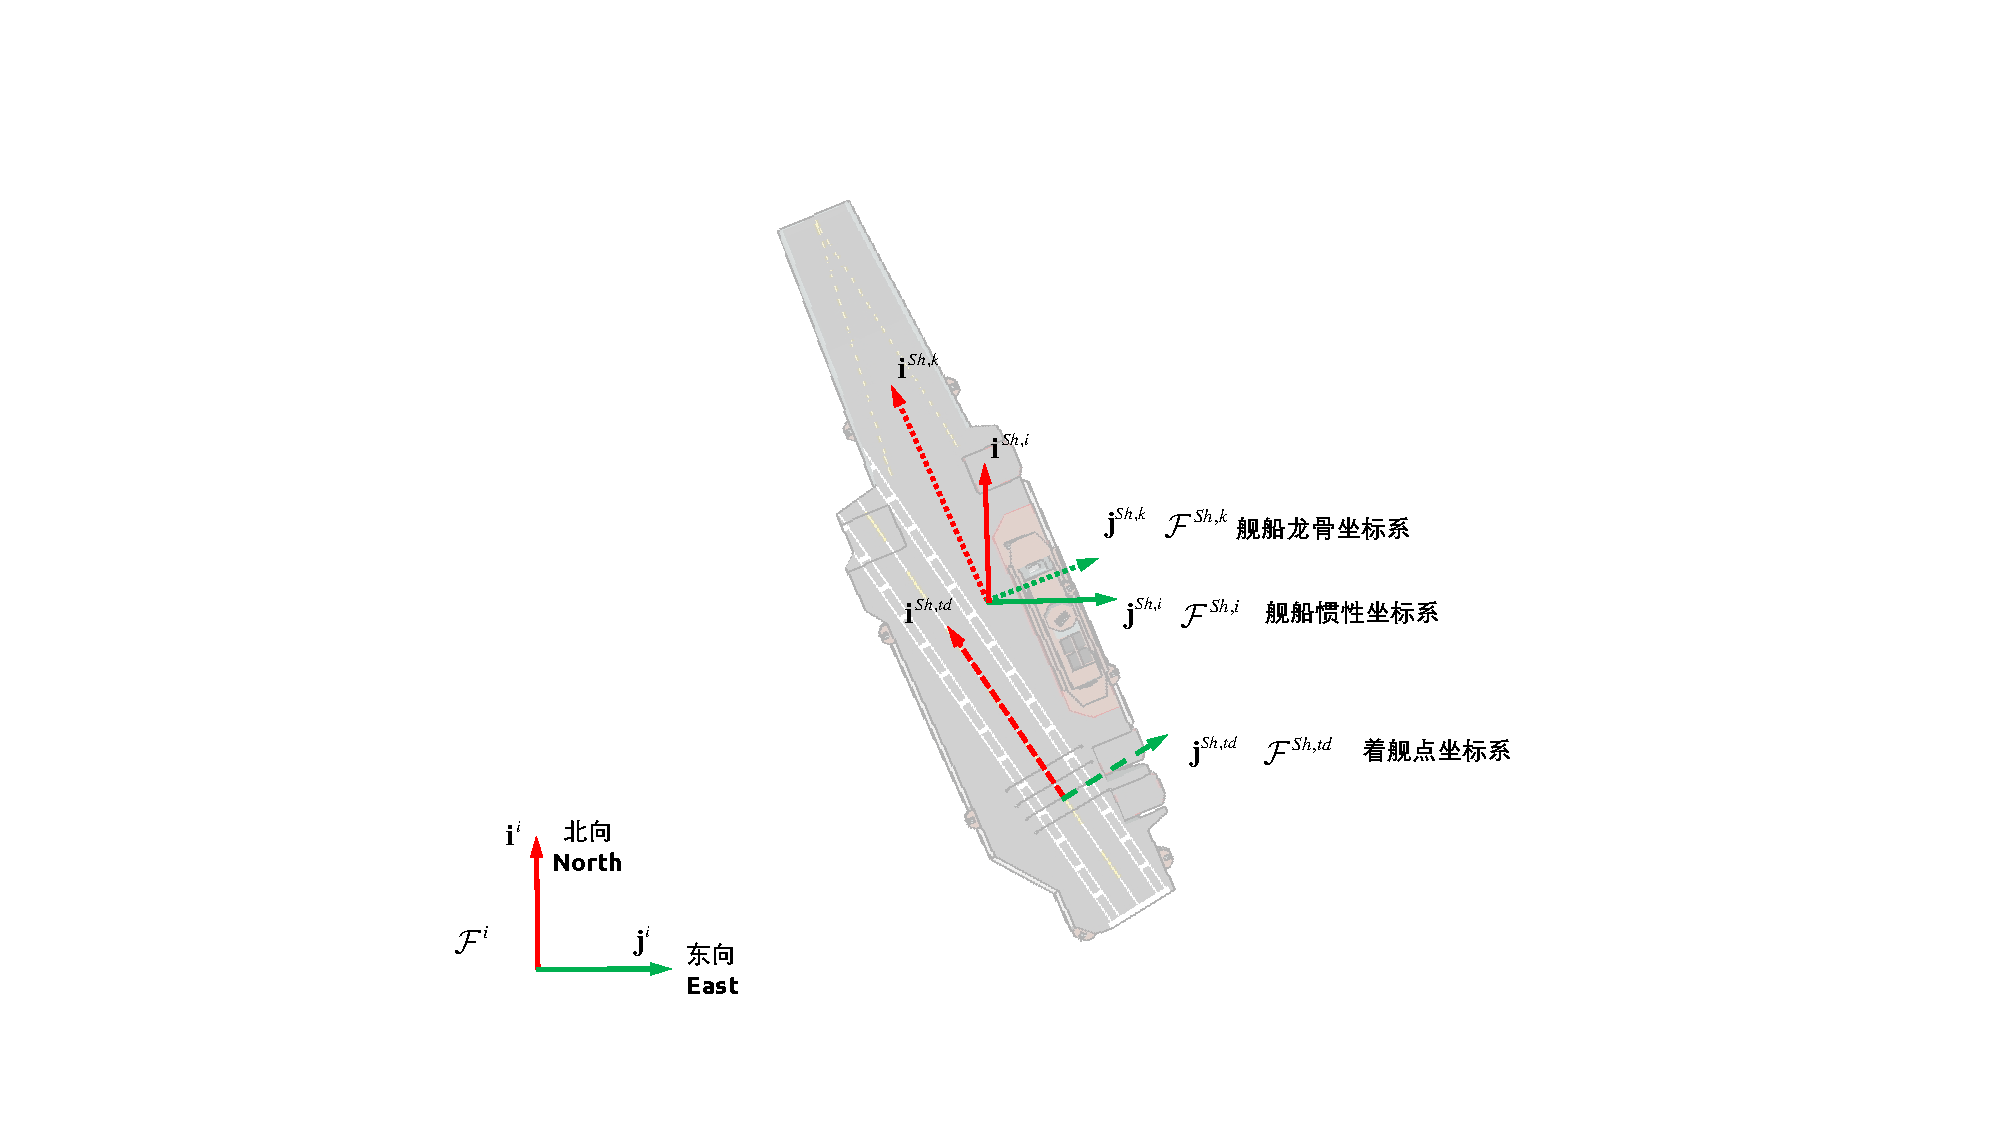
\includegraphics[width=0.8\textwidth]{figs/chp02/chp02_08_ship_interial_frame.pdf}
	\caption{舰船惯性坐标系}
	\label{fig:chp02_08_ship_interial_frame}
\end{figure}

\subsection{舰船龙骨坐标系}
舰船龙骨坐标系($\mathcal{F}^{Sh,k}$ ,Keel Frame),该坐标系的原点与舰船惯性坐标系相同,$\mathbf{i}^{Sh,k}$轴沿龙骨方向指向舰船前进方向,$\mathbf{j}^{Sh,k}$轴垂直于$\mathbf{i}^{Sh,k}$方向。因为该坐标系与船体固连,所以海浪的作用下,该坐标系随船体运动。与无人机机体坐标系类似,将舰船惯性坐标系按照3-2-1的顺序依次旋转至舰船龙骨坐标系,定义三次转动的角度为$\phi_{Sh}$、$\theta_{Sh}$和$\psi_{Sh}$,用于描述舰船的俯仰角、横滚角和偏航角。不同海况情况下,舰船龙骨坐标系还会存在周期性的扰动,由此定义$\Delta \phi_{Sh}$、$\Delta \theta_{Sh}$和$\Delta \psi_{Sh}$来描述舰船龙骨坐标系在俯仰、横滚和偏航三个轴线的扰动角度,定义$\Delta x_{surge}$、$\Delta y_{sway}$和$\Delta z_{heavy}$来描述三个坐标轴的位移偏差,即横摇、纵摇和沉浮。该坐标系的表达如图\ref{fig:chp02_09_ship_motion_frame}所示。

\begin{figure}[htb]   
	\centering
	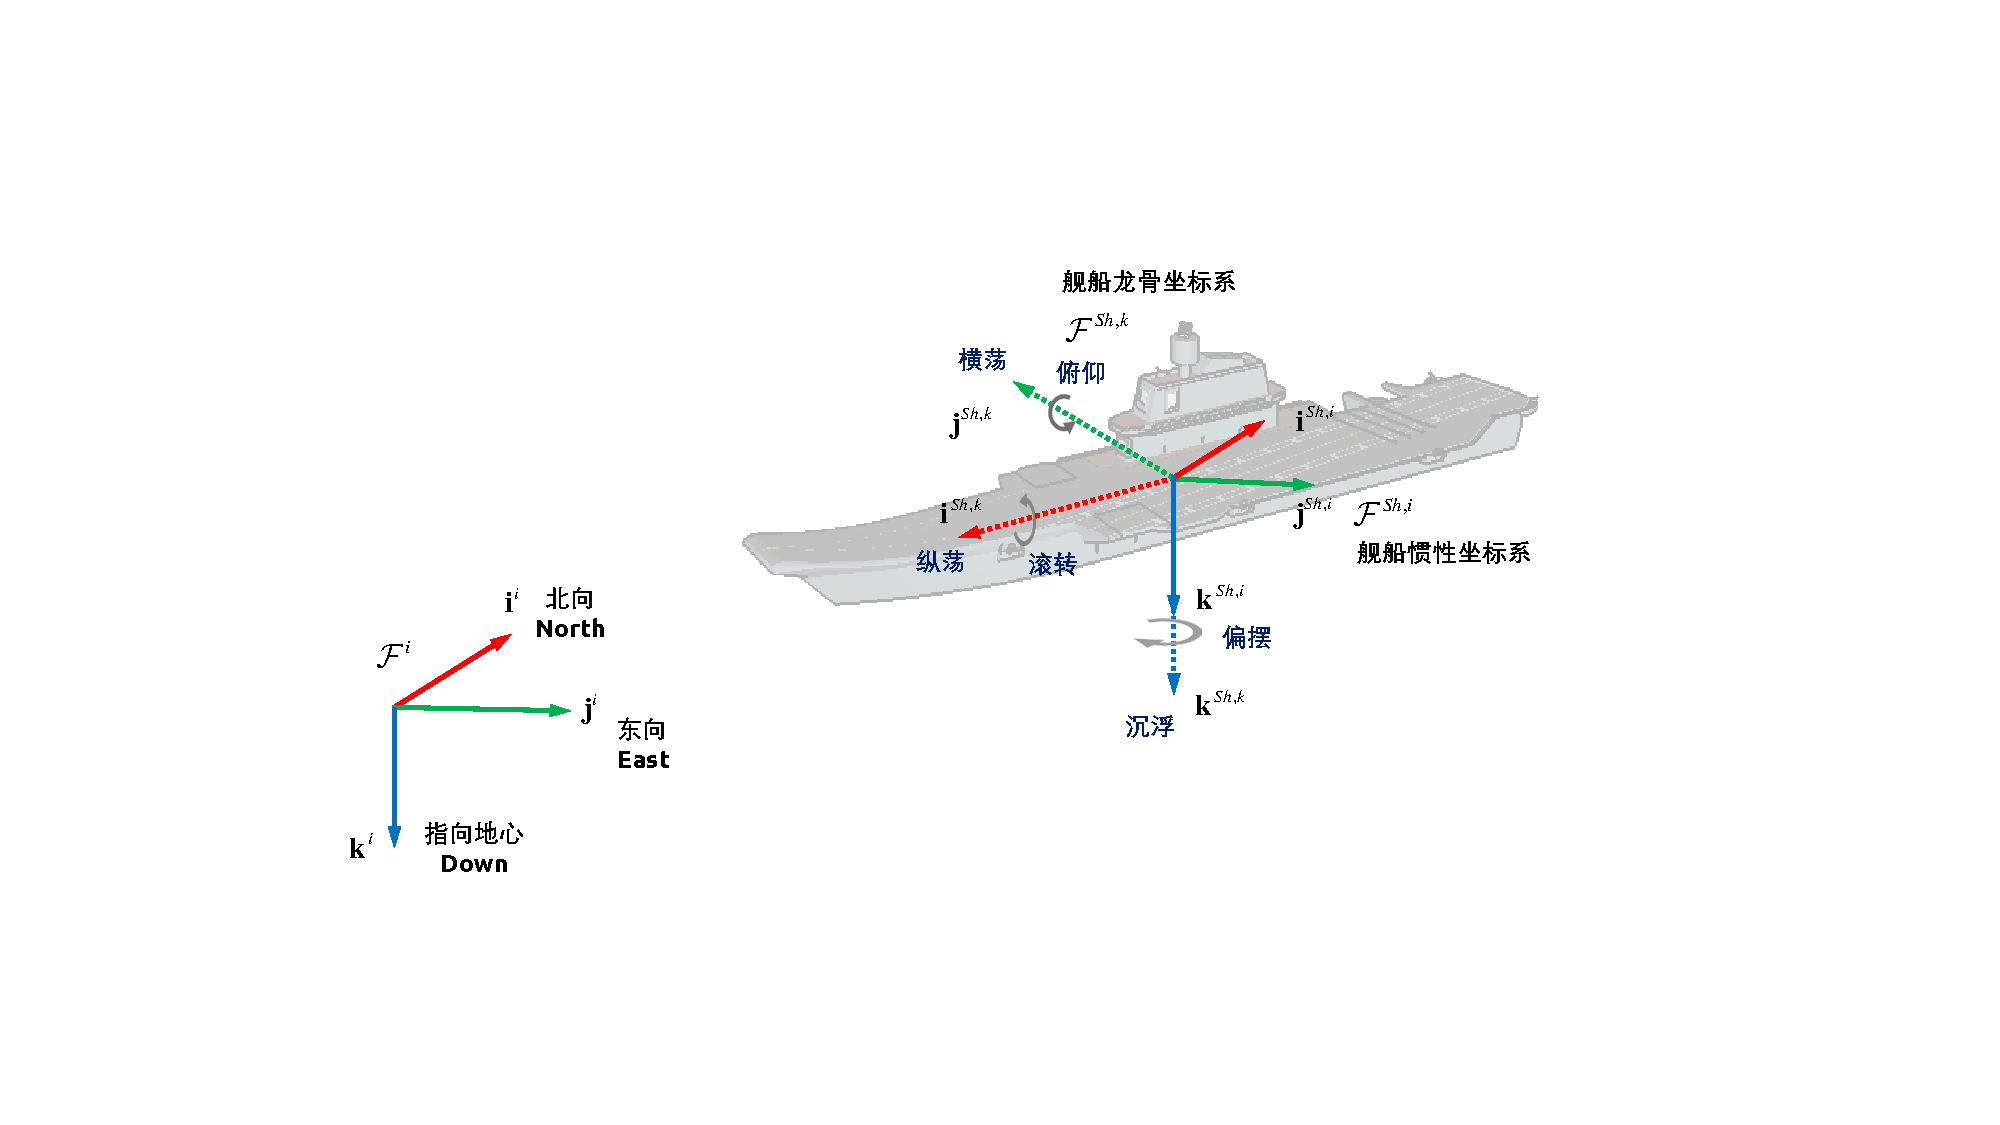
\includegraphics[width=\textwidth]{figs/chp02/chp02_09_ship_motion_frame.pdf}
	\caption{舰船系统坐标系的表达}
	\label{fig:chp02_09_ship_motion_frame}
\end{figure}


\subsection{着舰点坐标系}
着舰点坐标系($\mathcal{F}^{Sh,td}$,Touchdown Frame),该坐标系原点定义在第二条拦阻索的中间位置,$\mathbf{i}^{Sh,td}$轴沿降落跑道指向舰船运行前方,$\mathbf{j}^{Sh,td}$轴沿第二条拦阻索方向延长垂直于$\mathbf{i}^{Sh,td}$轴。

着舰点坐标系与舰船龙骨坐标系之间的转换关系定义为
\begin{equation}
	\begin{bmatrix} x_{Sh,td} \\ y_{Sh,td} \\z_{Sh,td} \end{bmatrix} = \begin{bmatrix} x_{Sh,k} \\ y_{Sh,k} \\z_{Sh,k} \end{bmatrix} +\mathcal{R}_{Sh,k}^{Sh,td} \begin{bmatrix} \Delta x_{Sh,k}^{Sh,td} \\ \Delta y_{Sh,k}^{Sh,td} \\ \Delta z_{Sh,k}^{Sh,td} 
	\end{bmatrix}
\end{equation}
其中$\Delta x_{Sh,k}^{Sh,td}$,$\Delta y_{Sh,k}^{Sh,td}$和$\Delta z_{Sh,k}^{Sh,td}$是着舰坐标系原点在舰船龙骨坐标系的坐标,$\mathcal{R}_{Sh,k}^{Sh,td}$是从舰船坐标系旋转到着舰点坐标系的旋转矩阵,该旋转矩阵的表达形式与无人机机体惯性坐标系转换到无人机机体坐标系的旋转矩阵相同,$(x_{Sh,k}\ y_{Sh,k}\ z_{Sh,k})$是舰船惯性坐标系上一点,该点在舰船着舰点坐标系上的坐标为$(x_{Sh,td}\ y_{Sh,td}\ z_{Sh,td})$。


由于舰船的运动,对于降落过程中的无人机需要提供有效的局部导航数据,本文设计的舰载引导系统坐标系主要用于描述引导系统对无人机的测量和导航。
\subsection{引导系统坐标系}
引导系统坐标系(Guidance Coordination System, $\mathcal{O}_c$)该坐标系的原点位于左侧引导系统的转台转轴的中心,$\mathbf{i}^{O,c}$轴指向右侧引导系统,并与着舰点坐标系的$\mathbf{j}^{Sh,td}$轴平行,$\mathbf{j}^{O,c}$轴与跑道纵向平行,指向远端无人机方向。该坐标系在舰船运动过程中与甲板固连,与期望着舰点坐标系的位置保持不变。一般而言,对于无人机着舰而言,期望着舰点的位置位于第一道和第二道拦阻索之间,靠近第二道拦阻索,如图\ref{fig:chp02_10_guidance_sys}所示;对于无人机装网回收而言,期望降落位置一般位于无人机回收网的几何中心。
\begin{figure}[htb]   
	\centering
	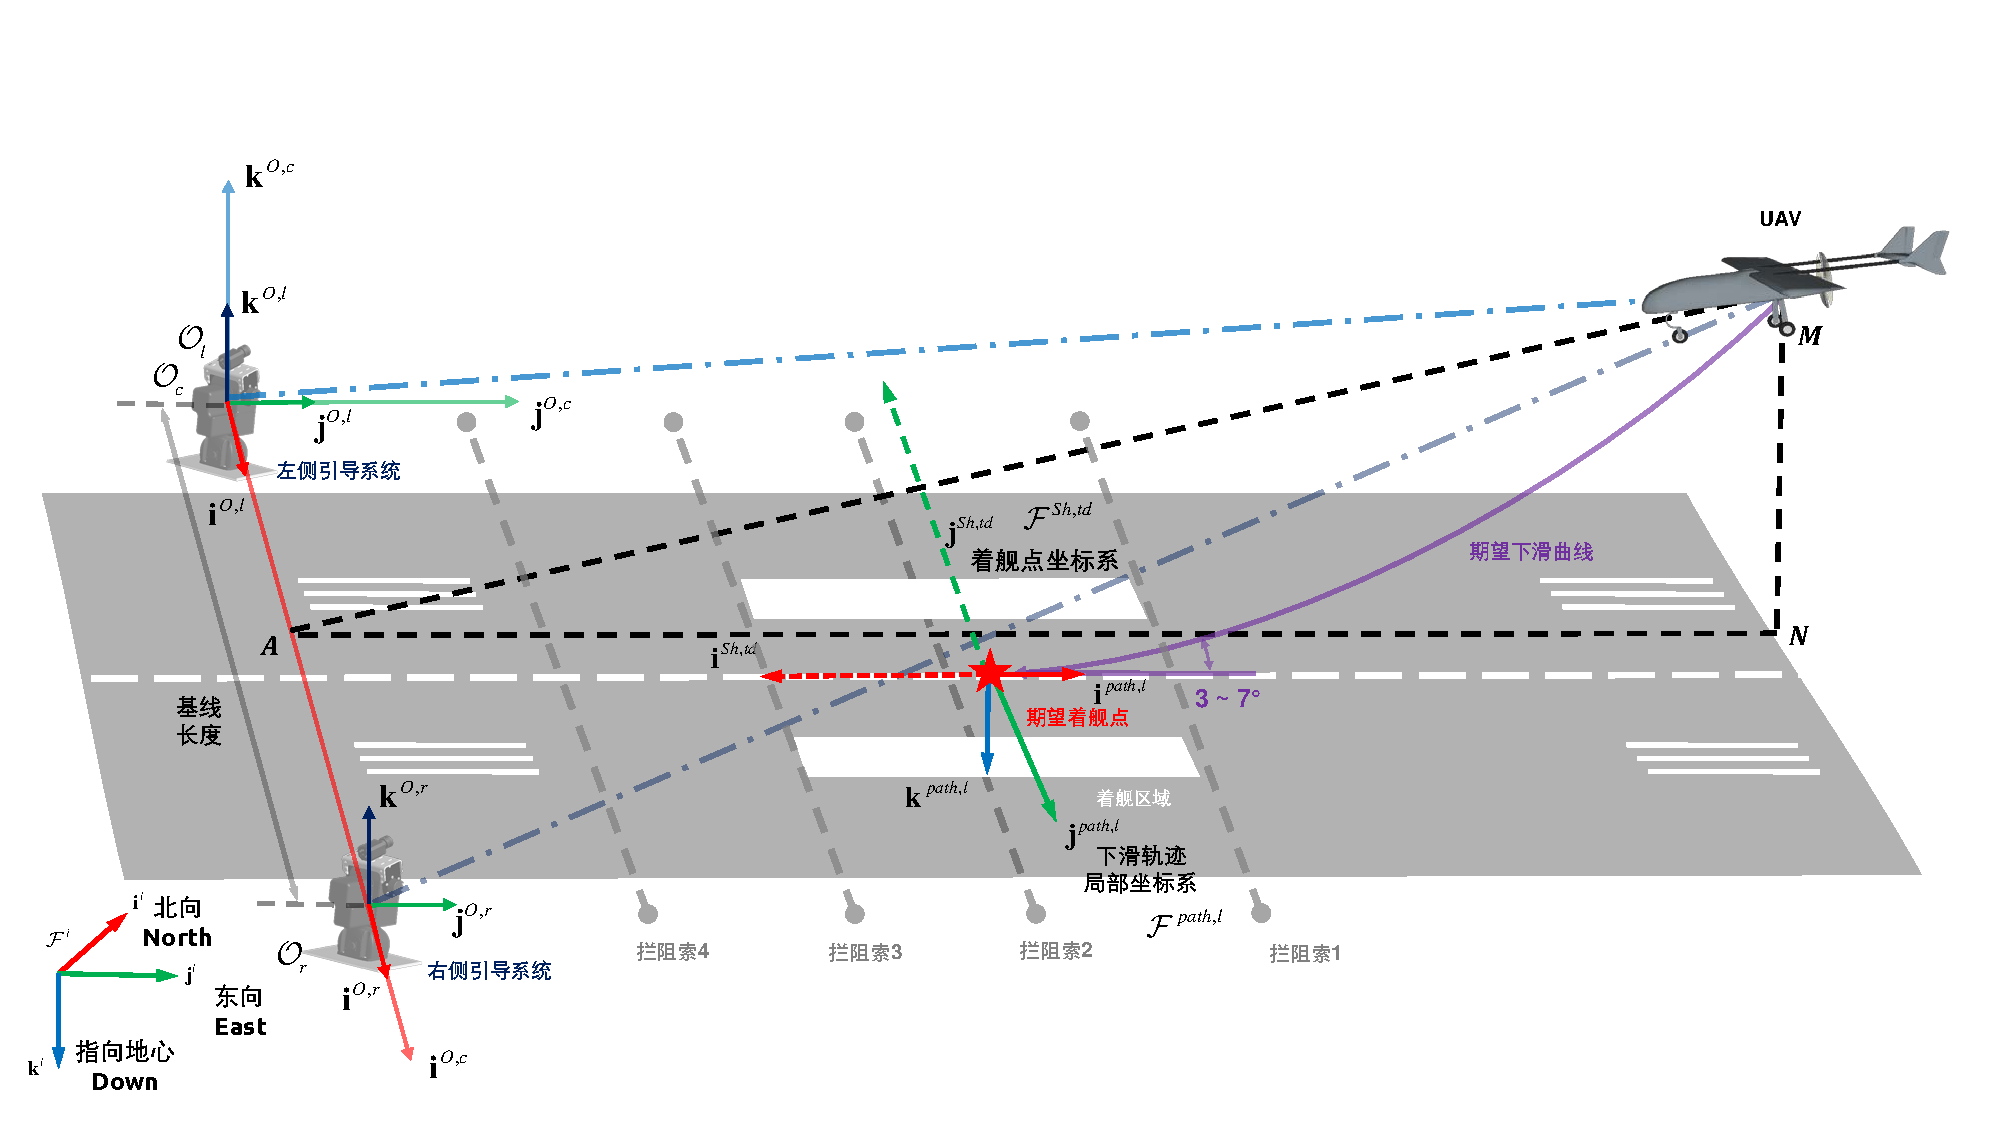
\includegraphics[width=\textwidth]{figs/chp02/chp02_10_guidance_sys.pdf}
	\caption{舰载引导系统相关坐标系}
	\label{fig:chp02_10_guidance_sys}
\end{figure}

\subsection{左右引导单元坐标系}
左侧引导系统坐标系($\mathcal{O}_l$)和右侧引导系统坐标系($\mathcal{O}_r$),这两个坐标系的原点别位于左侧和右侧引导系统的转台转轴中心,三个坐标轴的方向分别与光学引导系统相同。该引导单元坐标系也是用于立体解算无人机空间位置的主要坐标系。

\subsection{地心地固坐标系}
地心地固坐标系(Earth-Centered Earth-Fixed Coordinate System (ECEF),$\mathcal{O}_e$),该坐标系采用1984年\cite{WGS84}指定的地心空间右手坐标系(The World Geodetic System (WGS-84)),原点位于地球中心,$x$轴指向地球0°经线和0°纬线的交叉点,$y$轴指向地球的北极点。该坐标系通常用于大地测量、地图绘制和导航。本文后续试验中使用的该坐标系相关参数为 $R_{Ea}=6,378,137.0\ m$,$R_{Eb} = 6,356,752.0\ m$ ,$f=1/298.257223563$ 和 $e=0.08181919$。

\subsection{GPS坐标系}
GPS坐标系(The Geodetic Coordination System,$\mathcal{O}_g$)中的任意一点通常用$(\lambda\ \varphi\ h)$表示,其中 $\lambda$ 表示目标当前位置的经度, $\varphi$ 表示目标当前位置的纬度, $h$ 表示当前位置的高度。该数值一般通过GPS解算模块获得。

\subsection{GPS坐标系与地心地固坐标系之间的转换关系}
定义GPS经纬坐标系中任意一点$\mathbf{P}^g=(\lambda, \varphi, h)$,该点在地心地固坐标系的表达为

\begin{equation}
	\textbf{P}^e
	=
	\left[\begin{array}{c}
		X_e\\
		Y_e\\
		Z_e\\
	\end{array}\right]
	=
	\left[\begin{array}{c}
		(N_E+h)\cos \varphi \cos \lambda\\
		(N_E+h)\cos \varphi \sin \lambda\\
		(N_E(1-e^2)+h)\sin \varphi\\
	\end{array}\right]
\end{equation}

其中$N_E$是基于当前纬度位置的参数,根据上文所述的相关参数,该数值通常通过下式进行计算。

\begin{equation}
	N_E=\frac{R_{Ea}}{\sqrt{1-e^2 \sin^2 \varphi}}.
\end{equation}

\subsection{地心地固坐标系与系统惯性坐标系之间的转换关系}
定义系统惯性系原点在地心地固坐标系的原点为$\mathbf{P}_0^e(x_0\ y_0\ z_0)$,该点的GPS经纬坐标为$\mathbf{P}_0^g(\lambda_0\ \varphi_0\ h_0)$,地心坐标系中任意一点$\mathbf{P}^e$在系统惯性坐标系的表达为

\begin{equation}
	\textbf{P}^i=\mathcal{R}_e^n(\textbf{P}^e - \textbf{P}_0^e)
\end{equation}

其中转换矩阵$\mathcal{R}_e^n$为

\begin{equation}
	\mathcal{R}_e^n=\left[\begin{array}{ccc}
		-\sin \varphi _{0} \cos \lambda _{0} & -\sin \varphi _{0} \sin \lambda _{0} & \cos \varphi _{0}  \\
		-\sin \lambda _{0}           &           \cos \lambda _{0}            &          0           \\
		-\cos \varphi _{0} \cos \lambda _{0} & -\cos \varphi _{0} \sin \lambda _{0} & -\sin \varphi _{0}
	\end{array}\right]
\end{equation}

\subsection{舰船惯性坐标系与引导坐标系之间的转换关系}
定义在舰船惯性坐标系中的一点为$\mathbf{P}^{Sh,i}(X_{Sh,i}\ Y_{Sh,i}\ Z_{Sh,i})$,该点对应在引导坐标系的坐标为$\mathbf{P}^{c}(X_c\ Y_c\ Z_c)$,这两点之间的转换关系可以通过平移和旋转运算$(X_{Sh,i}, Y_{Sh,i}, Z_{Sh,i})\xrightarrow{\textbf{R}_{Sh,i}^c,T}(X_c, Y_c, Z_c) $得到,其矩阵表达形式为

\begin{equation}
	\left[\begin{array}{c}
		X_{Sh,i}\\
		Y_{Sh,i}\\
		Z_{Sh,i}\\
	\end{array}\right]=\mathcal{R}_{Sh,i}^c
	\left[\begin{array}{c}
		X_{c}\\
		Y_{c}\\
		Z_{c}\\
	\end{array}\right]+T_{Sh,i}^c
\end{equation}
其中
\begin{equation}
	\mathcal{R}_{Sh,i}^c=\left[\begin{array}{ccc}
		r_{11} & r_{12} & r_{13} \\
		r_{21} & r_{22} & r_{23} \\
		r_{31} & r_{32} & r_{33} 
	\end{array}\right]
	\ \ 
	T_{Sh,i}^c=\left[\begin{array}{ccc}
		t_{Sh,i}^c\\
		t_{Sh,i}^c\\
		t_{Sh,i}^c\\
	\end{array}\right]
\end{equation}
理想情况下,舰船惯性坐标系与引导坐标系之间的几何关系可以通过定义旋转和平移量获得,但由于引导系统的安装误差,该矩阵通常通过外部标定方法得到。




\section{双目引导系统标定方法}
\subsection{DGPS标定方法基本原理}
根据第二章定义的着舰系统坐标系之间的关系,在理想情况下,$\mathcal{F}_{path,l}$坐标系的原点位于跑道中线的延长线上,其坐标轴$\mathbf{i}^{path,l}$、$\mathbf{j}^{path,l}$和$\mathbf{k}^{path,l}$分别与引导坐标系的$\mathbf{j}^{O,c}$, $\mathbf{i}^{O,c}$和$\mathbf{k}^{O,c}$平行。但实际情况下,上述平行关系很难保证,两个坐标系的关系通常存在转动关系,因此$\mathcal{F}_{path,l}$与$\mathcal{O}_c$直接的位置关系不能通过简单的平移进行计算得到。两个坐标系之间的转换关系,主要通过DGPS外部标定方法完成\cite{liao2009automatic}。该方法通过将DGPS传感器放置在远端多个位置,(如图\ref{fig:chp03_vision_17_multi_dgps}所示),通过调节左右两侧转台的位置,使得光心对准DGPS的接收天线(如图\ref{fig:chp03_vision_16_dgps_calibration}所示),得到相应的转角关系。这里假设白色的DGPS天线的几何中线点作为标定点的真实位置。

\begin{figure}[!th]
	\centering
	\includegraphics[width=\textwidth]{figs/chp03_stereo/chp03_vision_17_multi_dgps.pdf}	
	\caption{多个DGPS靶标标定示意图}
	\label{fig:chp03_vision_17_multi_dgps}
\end{figure}


\begin{figure}[htb]
	\centering
	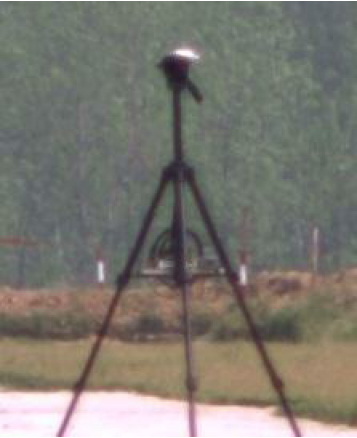
\includegraphics[width=0.4\textwidth]{figs/chp03_stereo/chp03_vision_16_dgps_calibration.pdf}	
	\caption{标定过程中,从左侧视觉系统中观察到的DGPS靶标}
	\label{fig:chp03_vision_16_dgps_calibration}
\end{figure}


相比于视觉系统的棋盘格标定方法,DGPS标定方法的优势是能够满足远距离标定需求。一般DGPS的设置点距离转台在$100\ m$以上,可以覆盖引导系统的末状态工作区域。而传统棋盘格由于制作尺寸受限,其标定范围一般在$5~10\ m$,该范围并不是转台经常工作的区域,其标定效果一般较差。

定义在下滑轨迹坐标系中任意一点的坐标为$(X_p, Y_p, Z_p)$,该点在引导坐标系的坐标系为$(X_c, Y_c, Z_c)$,因此需要求解这两个坐标系之间的转换矩阵
\begin{equation}
\left[ {\begin{array}{*{20}{c}}
	{{X_p}} \\ 
	{{Y_p}} \\ 
	{{Z_p}} 
	\end{array}} \right] = \mathcal{R}_c^p\left[ {\begin{array}{*{20}{c}}
	{{Z_{c}}} \\ 
	{{Y_{c}}} \\ 
	{{Z_{c}}} 
	\end{array}} \right] + T_c^p
\end{equation}
其中$\mathcal{R}_c^p$是$3\times3$旋转矩阵,$T_c^p$是$3\times1$平移矩阵。由于转换关系符合欧拉角定义,按照$\psi-\theta-\phi$的转换顺序,可以得到
\begin{equation}
\mathcal{R}_c^p = \begin{bmatrix}
\cos \theta \cos \psi                             & \cos\theta \sin\psi                               & -\sin\theta         \\
-\cos\phi \sin\psi + \sin\phi \sin\theta \cos\psi & \cos\phi \cos\psi + \sin\phi \sin\theta\sin\psi   & \sin\phi \cos\theta \\
\sin\phi \sin\psi + \cos\phi \sin\theta \cos\psi  & -\sin\phi \cos\psi + \cos\phi \sin\theta \sin\psi & \cos\phi \cos\theta
\end{bmatrix}
\end{equation}
上述转换矩阵中的欧拉角无法通过解析的方法求得,只能通过多次采集标定点数据最优迭代获得。因此,定义旋转矩阵和平移矩阵的分量为
\begin{equation}
\mathcal{R}_c^p = \begin{bmatrix}
r_{11} & r_{12} & r_{13}\\
r_{21} & r_{22} & r_{23}\\
r_{31} & r_{32} & r_{33}\\
\end{bmatrix}
\end{equation}

\begin{equation}
T_c^p=\left[ {\begin{array}{*{20}{c}}
	t_x \\ 
	t_y \\ 
	t_z 
	\end{array}} \right]
\end{equation}
当通过手动控制转台使得光心对准DGPS天线时,上述6个变量$(\phi\ \theta\ \psi\ t_x\ t_y\ t_z)$与转台角度俯仰角$\phi_l$和方位角$\psi_l$之间的关系为
\begin{equation}
\left\{ \begin{gathered}
\tan \phi_l = \frac{Y_p}{Z_p} \\
\tan \phi_l = \frac{X_p}{\sqrt{X_p^2+Z_p^2} }\\
\end{gathered}  \right.
\end{equation}

\begin{equation}
\left\{ \begin{gathered}
\tan \phi_l= \frac{r_{21}X_p + r_{22}Y_p + r_{23}Z_p + t_y}{r_{31}X_p + r_{32}Y_p + r_{33}Z_p + t_z} \\
\tan \psi_l= \frac{r_{11}X_p + r_{12}Y_p + r_{13}Z_p + t_y}{\sqrt{(r_{31}X_p + r_{32}Y_p + r_{33}Z_p + t_y)^2+(r_{21}X_p + r_{22}Y_p + r_{23}Z_p + t_y)^2} }\\
\end{gathered}  \right.
\end{equation}

二维转台DGPS方法标定的基本步骤如下:
\begin{compactenum}
	\item
	转台系统初始化,并归零。
	\item
	放置DGPS点在不同位置(不少于3组,一般为10组),并该点的DGPS数据和转台两个转动角度。
	\item
	将采集到的数据通过非线性最小二乘的方法求解得到上述6个标定参数。
\end{compactenum}
注意在标定过程中,尽可能保持DGPS横向($\mathbf{i}^{O,c}$轴向)移动的连续性,使得转台始终向一侧转动。由于转动机械机构的误差,转台出现连续向左和向右的运动,容易将误差放大。

\subsection{DGPS标定方法实验验证}
配置左右视觉单元的基线距离为$10\ m$,实验总共采集20组DGPS靶标数据,其中使用前10组数据进行参数的求解,使用后10组数据来验证上述标定方法的准确性。这些点选取的一般位于距离标定单元$100\ m$左右,尽可能覆盖转台方位角$-25\degree-25\degree$的范围,该标定区域的示意图如\ref{fig:chp03_vision_18_dgps_calibration_diagram}所示。其中一组标定数据集的系统标定参数如表\ref{label:dgps_calibration}所示。

\begin{figure}[htb]
	\centering
	\includegraphics[width=0.7\textwidth]{figs/chp03_stereo/chp03_vision_18_dgps_calibration_diagram.pdf}	
	\caption{DGPS标定过程中选定的20个标定点}
	\label{fig:chp03_vision_18_dgps_calibration_diagram}
\end{figure}

\begin{table}[htb]
	\centering
	\caption{DGPS标定方法得到的标定数据}
	\label{label:dgps_calibration}
	\begin{tabular}{ccccccc}
		\hline
		标定参数 & $\phi (\degree)$ & $\theta (\degree)$ & $\psi (\degree)$ & $t_x (m)$ & $t_y(m)$ & $t_z(m)$ \\ \hline
		实际数值 & 1.58             & -0.01              & 1.57             & -0.41     & 23.31   & -2.21    \\ \hline
	\end{tabular}
\end{table}

在得到上述标定参数后,通过后续10个测试数据来检验标定的精度。表\ref{label:DGPS_Pan_Tilit_Calibration_Error}是这是个测试DGPS点的真实值和解算值。其中,十组数据的方位角平均误差为$0.0141\degree$,俯仰角的平均误差为$-0.0319\degree$。每个标定点的误差曲线如图\ref{fig:chp03_vision_19_pan_tilt_ten_points_error}所示。

% /home/amax/Workspace/77.GOTURN/GOTURN/landing_original_folder/Landing_Data_1
\begin{table}[]
	\centering
	\caption{DGPS标定测试集误差}
	\label{label:DGPS_Pan_Tilit_Calibration_Error}
	\begin{tabular}{crrrr}
		\hline
		& \multicolumn{2}{c}{真实值$(\degree)$}                           & \multicolumn{2}{c}{标定值$(\degree)$}                           \\ \hline
		DGPS点编号 & \multicolumn{1}{c}{方位角} & \multicolumn{1}{c}{俯仰角} & \multicolumn{1}{c}{方位角} & \multicolumn{1}{c}{俯仰角} \\ \hline
		1       & 0.7843                  & -0.0836                 & 0.7730                  & -0.0691                 \\
		2       & 5.9854                  & 0.5722                  & 6.0372                  & 0.6129                  \\
		3       & 0.9065                  & 0.5722                  & 0.8573                  & 0.6404                  \\
		4       & -4.5582                 & 0.4757                 & -4.5237                 & 0.5322                  \\
		5       & -4.7832                 & 0.1350                  & -4.7748                 & 0.1343                  \\
		6       & 1.7294                  & 1.0094                  & 1.6185                  & 1.0921                  \\
		7       & 8.1520                  & 1.1122                  & 8.0970                  & 1.1053                  \\
		8       & -5.1689                 & 1.1701                  & -5.2517                 & 1.2527                  \\
		9       & 3.6645                  & 0.4307                  & 3.6734                  & 0.4075                  \\
		10      & -3.6388                 & 0.4565                  & -3.5739                 & 0.4614                  \\ \hline
	\end{tabular}
\end{table}


\begin{figure}[htb]
	\centering
	\includegraphics[width=\textwidth]{figs/chp03_stereo/chp03_vision_19_pan_tilt_ten_points_error.pdf}	
	\caption{DGPS标定测试集方位角和俯仰角误差曲线}
	\label{fig:chp03_vision_19_pan_tilt_ten_points_error}
\end{figure}

为了验证该标定方法的有效性,重复上述实验10次,得到的标定误差结果如表\ref{label:DGPS_10_Test_Results}所示。其中10组测试中两个角度的最大误差用粗体表示。通过实验可以看到,该方法的标定精读较高,能够满足坐标系转换需求。
\begin{table}[htb]
	\centering
	\caption{10组DGPS标定方法测试俯仰角和方位角误差}
	\label{label:DGPS_10_Test_Results}
	\begin{tabular}{crr}
		\hline
		实验组数 & \multicolumn{1}{c}{方位角误差平均值} & \multicolumn{1}{c}{俯仰角俯仰角误差平均值} \\ \hline
		1    & 0.0141                       & -0.0319                         \\
		2    & \textbf{-0.0211}             & 0.0221                          \\
		3    & 0.0085                       & -0.0322                \\
		4    & -0.0133                      & -0.0149                         \\
		5    & -0.0093                      & 0.0350                          \\
		6    & 0.0043                       & -0.0132                         \\
		7    & -0.0132                      & 0.0152                          \\
		8    & -0.0201                      & -0.0320                         \\
		9    & 0.0114                       & -0.0119                         \\
		10   & -0.0147                      & \textbf{0.0565}                          \\ \hline
	\end{tabular}
\end{table}




\section{本章小结}
本章根据无人机着舰过程中的需求,系统定义了无人机和舰船两大类坐标系,并根据各自系统的数学推算需要,定义了引导坐标系、下滑轨迹坐标系、风向坐标系等。上述小节对相关重点坐标系的符号定义和对相互转换关系进行推导。




